\chapter{Experimentos e resultados}
\label{chap:Experimentos e resultados}
\lettrine{N}{este} capítulo presentaranse os experimentos realizados e os resultados obtidos.
Para iso, comezarase presentando unha vista xeral do proceso de experimentación, 
seguido dos propios experimentos realizados, para 
Finalmente analizar os resultados obtidos en conxunto e as conclusións que se poden extraer deles.

\section{Vista Xeral}
\label{sec:Vista Xeral}

O obxetivo do traballo é determinar se as redes implícitas son aptas para a tarefa de rexistro de retinas.
Aínda que partimos do traballo de IDIR, a tarefa de rexistro de retinas presenta diferenzas importantes respecto ao rexistro de pulmóns. Por este motivo, non podemos asumir que os parámetros óptimos para pulmóns sexan tamén os mellores para retinas.

Ao longo dos experimentos, a comparación principal céntrase na función de activación empregada (SIREN ou ReLU).
Debido ao gran espazo de búsqueda que implica probar todas as configuracións posibles, 
os experimentos iniciais centraránse en fixar unha unha seria de parámetros con valores razoables para poder experimentar só con aqueles que teñan un impacto máis significativo.

Ademais, debido ás diferencias entre as funcións de activación, é posible que cada unha require unha configuración diferente para obter os mellores resultados.
Por exemplo, o sesgo que SIREN ten cara sinais de alta frecuencia fará que o proceso de regularización sexa mais relevante para evitar o sobreaxuste.

\section{Experimentos}
\label{sec:Experimentos}

\subsection{Experimentos iniciais}
\label{subsec:Experimentos iniciais}

Inicialmente tentaremos determinar uns valores aceptables para varios dos parámetros da rede.
Isto é relevante xa que moitos destes parámetros son dependentes uns de outros.

A menos que especificado de outro xeito, os parámetros utilizados para os experimentos son os seguintes:
\begin{itemize}
    \item Función de perda: NCC
    \item Regularización:
    \begin{itemize}
         \item Bending energy penalty: 10.0
         \item Jacobian regularizer: 0.05
         \item Hyperelastic regularizer: 0.25
    \end{itemize}
    \item Learning rate: 0.0001
    \item Batch size: 10000 puntos
    \item Epochs: 1500
    \item Optimizador: Adam
    \item Resolución: 1000x1000
\end{itemize}


\subsubsection{Función de loss}
\label{subsubsec:Función de loss}

\paragraph{Planteamento}
\label{par:Planteamento}

A función de loss é un dos aspectos máis importantes á hora de entrenar unha rede neuronal.
As funcións de perda valoradas para este traballo xa forón explicadas en \ref{subsubsec:Termos de loss}.

Para determinar cal é a función de perda mais adecuada para a tarefa de rexistro de retinas, realizáronse experimentos comparando o rendemento de cada unha sobre unha mostra de imaxes dos datases de FIRE e RFMID.
Xa que a rede non é capaz de rexistrar con éxito a gran parte das imaxes, tomaráse a distancia media de todos os puntos como métrica de comparación.

\paragraph{Resultados}
\label{par:Resultados}

Os resultados obtidos son os seguintes: \ref{tab:mean_distances}, \ref{fig:loss_functions_comparison}

% \begin{table}[h]
%     \centering
%     \begin{tabular}{|l|c|c|}
%     \hline
%     Loss Function & FIRE Mean Distance & RFMID Mean Distance \\ \hline
%     ncc & 250.59 & 36.04 \\ \hline
%     mse & 392.94 & 9.50 \\ \hline
%     l1 & 404.83 & 5.42 \\ \hline
%     smoothl1 & 414.79 & 7.01 \\ \hline
%     \end{tabular}
%     \caption{Distancias medias según a función de perda. Valores máis baixos son mellores.}
%     \label{tab:mean_distances}
% \end{table}


\begin{table}[h]
    \centering
    \begin{tabular}{|l|cc|cc|}
    \hline
    \multirow{2}{*}{Loss Function} & \multicolumn{2}{c|}{FIRE Dataset} & \multicolumn{2}{c|}{RFMID Dataset} \\ \cline{2-5}
     & Relu & SIREN & Relu & SIREN \\ \hline
    huber & 399.86 & 397.45 & 7.13 & 57.31 \\ \hline
    l1 & 404.83 & 391.87 & 5.42 & 52.91 \\ \hline
    mse & 392.94 & 410.97 & 9.50 & 121.54 \\ \hline
    ncc & 250.59 & 281.03 & 36.04 & 79.84 \\ \hline
    smoothl1 & 414.79 & 387.71 & 7.01 & 60.74 \\ \hline
    ssim & 268.72 & 264.98 & 23.34 & 55.07 \\ \hline
    \end{tabular}
    \caption{Distancias medias segundo función de perda, tipo de rede e datasets (FIRE vs. RFMID)}
    \label{tab:mean_distances}
\end{table}

\begin{figure}[h]
    \centering
    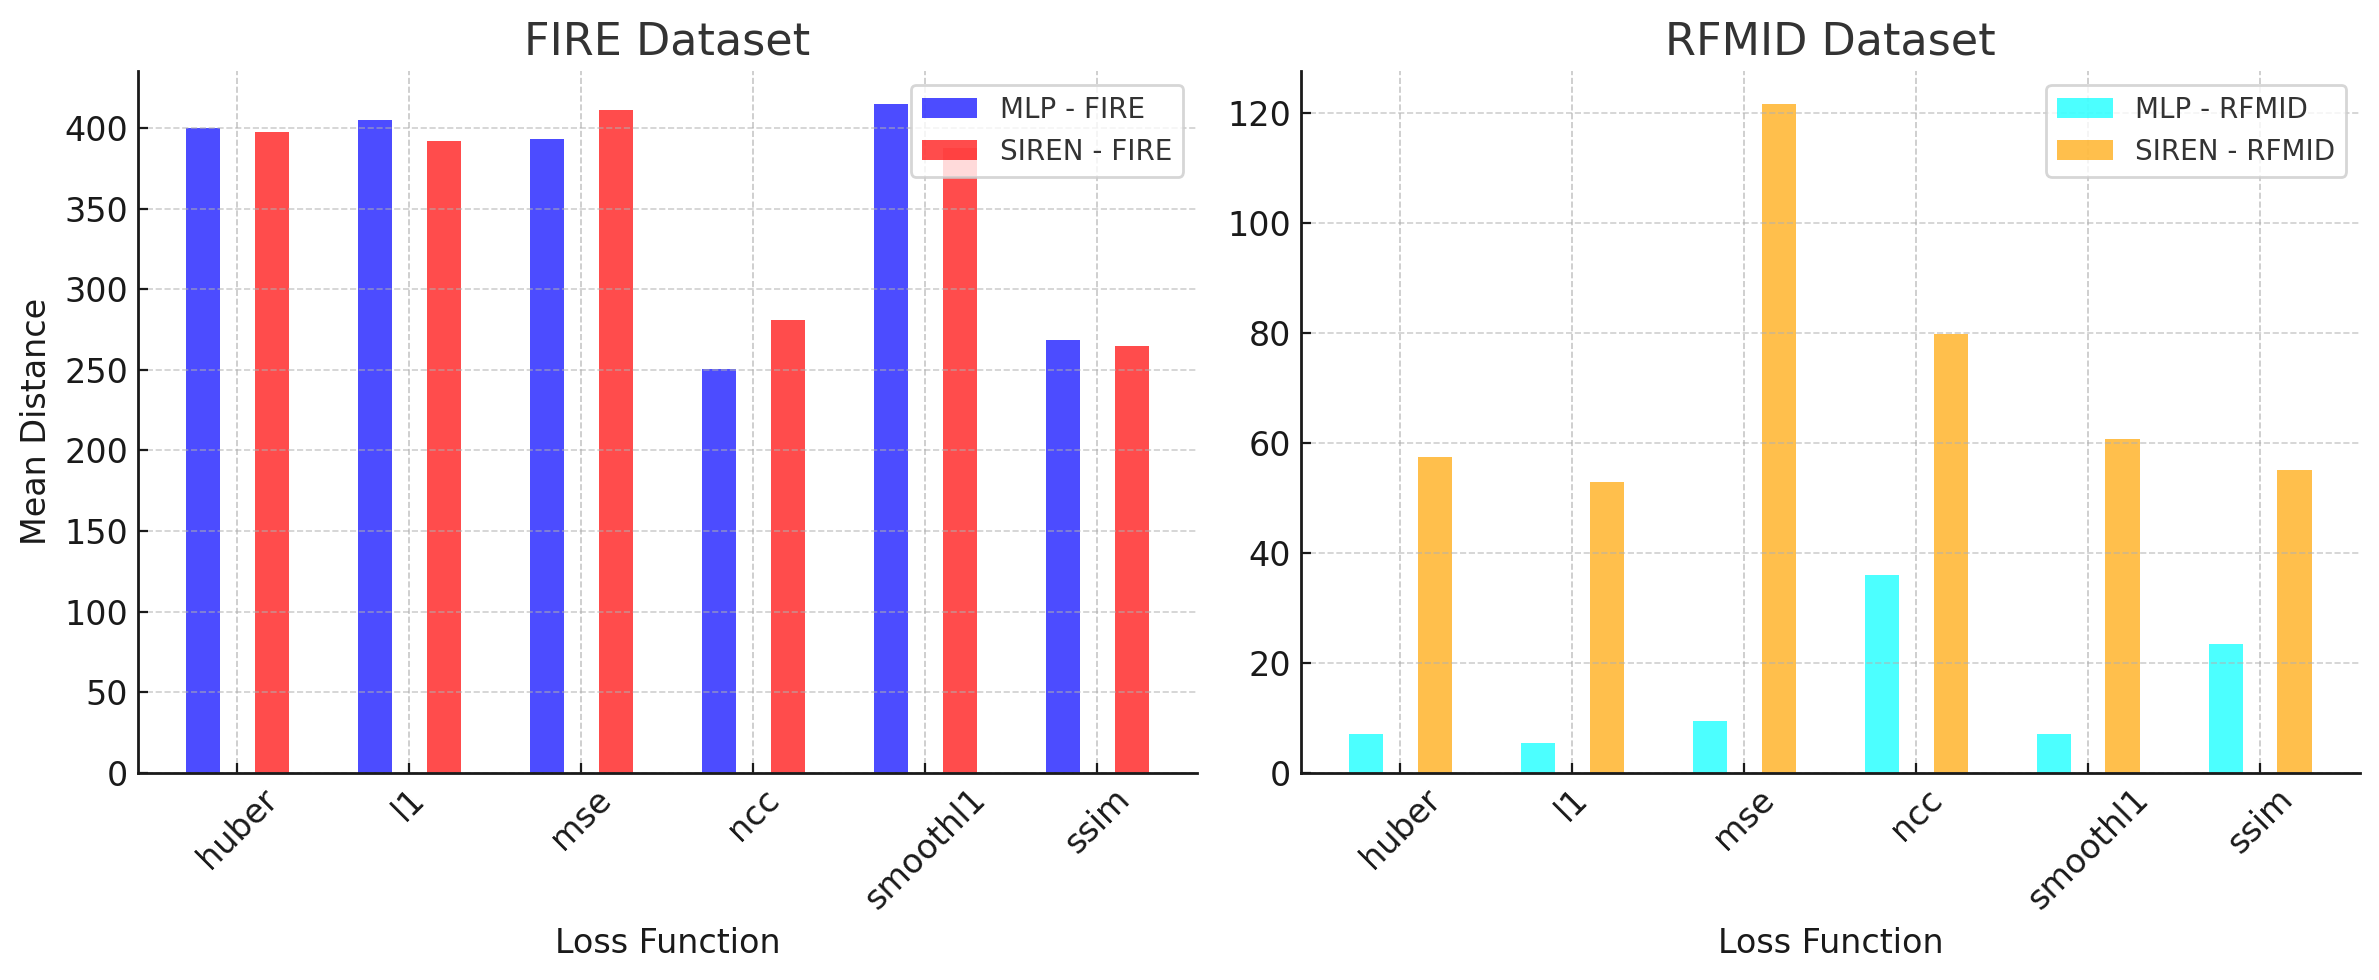
\includegraphics[width=0.75\textwidth]{imaxes/losstype.png}
    \caption{Comparación de diferentes funcións de perda sobre imaxes de FIRE e RFMID}
    \label{fig:loss_functions_comparison}
\end{figure}
    


\paragraph{Discusión}
\label{par:Discusión}

Obsérvase como as métricas que teñen en conta a estructura da imaxe (NCC, SSIM) tenden a dar mellores resultados que aquelas que non o fan (MSE, Huber, Smooth L1) co dataset de FIRE, mentres que con RFMID ocurre ó contrario.
Isto pode deberse a que as imaxes reais de retina teñen unha maior variabilidade na iluminación e contraste, polo que as métricas que non teñen en conta a estructura da imaxe serán menos robustas a estas diferenzas.
No caso de RFMID, ao ser imaxes sintéticas, a variabilidade na iluminación e contraste é nula, o que explica os mellores resultados das métricas que non teñen en conta a estructura da imaxe.

NCC tende a ser mais robusta a combios uniformes na intensidade global, mentres que SSIM tende a ser mellor con cambios locais.
SSIM tamén é menos robusta ao ruído, sensible o tamaño das seccións utilizadas e computacionalmente mais costosa. Ademais, ten outro custo engadido xa que non é posible calcular SSIM tan só comparando os puntos mostrados xa que utiliza xanelas deslizantes para evaluar luminancia, contraste e estrutura. 
Para utilizala é necesario reconstruir a imaxen en cada iteracion o que ten un alto custo computacional.
No caso de non reconstruir a imaxe e utilizar os puntos mostrados directamente, esta métrica funciona igualmente mais con resultados lixeiramente peores, xa que perde toda a súa capacidade de capturar variacións locais de luminancia, contraste e estrutura, o que se tradúce nunha función de perda global sen consideraciós locais.

\paragraph{Conclusións}
\label{par:Conclusións}

En base aos resultados obtidos, pódense extraer varias conclusións relevantes:

1. Para o dataset FIRE, que contén imaxes reais de retina con variabilidade en iluminación e contraste, as funcións de perda baseadas en características estruturais como NCC e SSIM proporcionan resultados significativamente mellores. En particular, NCC mostra o menor erro medio (250.59 para Relu e 281.03 para SIREN).
2. Para o dataset RFMID, que contén imaxes con tan só variación xeométrica, as funcións de perda baseadas en píxeles como L1 e Smooth L1 ofrecen mellores resultados. Concretamente, L1 presenta o menor erro medio para Relu (5.42) e resultados competitivos para SIREN (52.91).
3. Obsérvase unha diferenza sistemática entre os modelos Relu e SIREN, sendo os primeiros máis efectivos para o dataset RFMID, mentres que ambos mostran rendementos comparables para FIRE. Isto débese a que Relu tende a producir funcións predominantemente lineares, o que se adapta mellor ás transformacións realizadas no dataset RFMID.
4. SSIM, a pesar de ser teoricamente robusta a cambios locais, non mostra unha vantaxe significativa sobre NCC.

A elección de NCC como función de perda estándar baséase tanto na súa robustez empírica coma na súa consistencia co obxectivo de alinear imaxes reais de retina, onde a variabilidade en iluminación e contraste é un factor importante.

\subsubsection{Resolución da imaxe}
\label{subsubsec:Resolución da imaxe}

\paragraph{Planteamento}
\label{par:Planteamento}

A resolución da imaxe é un aspecto clave xa que inflúe de forma directa no resto de parámetros da rede.
Por exemplo, un batch size de 1000 puntos nunha imaxe de 256x256 é unha densidade de puntos moito maior que nunha imaxe de 512x512.

Ademais, a resolución da imaxe tamén inflúe na capacidade da rede para aprender as transformacións, xa que a información que recibe é mais detallada. 
Isto pode ser beneficioso se estos detalles conteñen información relevante para a tarefa de rexistro, pero tamén podería ser perxudicial se conteñen unha gran parte de ruido.

O tamaño das imaxes tamén é unha das principais diferencias entre as imaxes de retina e as de pulmóns utilizadas orixinalmente por IDIR, tendo estas últimas de 512x512 mentres que as imaxes dos ollos contan con resolucións de ata 2160x2160.

Para determinar cal é a resolución mais adecuada, realizáronse experimentos comparando o rendemento de cada unha sobre unha mostra de imaxes dos datases de FIRE e RFMID.
Debido a que a rede non é capaz de rexistrar con éxito a gran parte das imaxes, tomaráse a distancia media de todos os puntos como métrica de comparación.

\paragraph{Resultados}
\label{par:Resultados}

\ref{tab:mlp_mean_distances_fire}, \ref{tab:siren_mean_distances_fire}, \ref{tab:mlp_mean_distances_rfmid}, \ref{tab:siren_mean_distances_rfmid}

\begin{table}[h]
    \centering
    \begin{minipage}[t]{0.45\linewidth}
        \centering
        \begin{tabular}{|c|c|}
        \hline
        Resolution & Mean Distance \\ \hline
        100 & 254.22 \\ \hline
        250 & 251.29 \\ \hline
        750 & 250.62 \\ \hline
        1250 & 250.59 \\ \hline
        1708 & 249.72 \\ \hline
        \end{tabular}
        \caption{Distancias medias para o dataset FIRE ca función de activación Relu}
        \label{tab:mlp_mean_distances_fire}
    \end{minipage}
    \hfill
    \begin{minipage}[t]{0.45\linewidth}
        \centering
        \begin{tabular}{|c|c|}
        \hline
        Resolution & Mean Distance \\ \hline
        100 & 266.43 \\ \hline
        250 & 263.85 \\ \hline
        750 & 263.19 \\ \hline
        1250 & 258.56 \\ \hline
        1708 & 258.06 \\ \hline
        \end{tabular}
        \caption{Distancias medias para o dataset FIRE ca función de activación SIREN}
        \label{tab:siren_mean_distances_fire}
    \end{minipage}
\end{table}

\begin{table}[h]
    \centering
    \begin{minipage}[t]{0.45\linewidth}
        \centering
        \begin{tabular}{|c|c|}
        \hline
        Resolution & Mean Distance \\ \hline
        100 & 37.29 \\ \hline
        250 & 36.18 \\ \hline
        750 & 36.01 \\ \hline
        1250 & 35.03 \\ \hline
        1708 & 35.04 \\ \hline
        \end{tabular}
        \caption{Distancias medias para o dataset RFMID ca función de activación Relu}
        \label{tab:mlp_mean_distances_rfmid}
    \end{minipage}
    \hfill
    \begin{minipage}[t]{0.45\linewidth}
        \centering
        \begin{tabular}{|c|c|}
        \hline
        Resolution & Mean Distance \\ \hline
        100 & 68.12 \\ \hline
        250 & 73.42 \\ \hline
        750 & 77.55 \\ \hline
        1250 & 67.33 \\ \hline
        1708 & 67.31 \\ \hline
        \end{tabular}
        \caption{Distancias medias para o dataset RMIFD ca función de activación SIREN}
        \label{tab:siren_mean_distances_rfmid}
    \end{minipage}
\end{table}

\paragraph{Discusión}
\label{par:Discusión}

Pódese observar como unha maior resolución tende a dar lixeiramente mellores resultados, pero a un custo computacional maior.
Isto pode deberse mais á precisión ca que se fai a evaluación mais que a unha mellor capacidade da rede para aprender as transformacións, xa que as diferencias son moi pequenas e consistentes entre os diferentes parellas de imaxes.
Isto suxire que a resolución non ten un impacto significativo no rendemento da rede, e que a maioría da información relevante para a tarefa de rexistro xa está capturada en resolucións inferiores.


\paragraph{Conclusións}
\label{par:Conclusións}

Baseándonos nos resultados obtidos, podemos concluír que:

1. Resolucións inferiores a 100×100 non capturan suficientes detalles das estruturas vasculares retinianas para realizar un rexistro preciso, especialmente en imaxes reais do dataset FIRE.

2. Aumentar a resolución por encima de 1250x1250 non aporta beneficios significativos.

3. O comportamento respecto á resolución é consistente para ambos tipos de modelos (Relu e SIREN) e para ambos datasets (FIRE e RFMID), o que suxire que estas conclusións son xeneralizables.

Para os experimentos subseguintes, adoptarase unha resolución estándar de 1000x1000 píxeles, que demostrou proporcionar o mellor rendemento global para a tarefa de rexistro de retinas.

\subsubsection{Regularización}
\label{subsubsec:Regularización}

\paragraph{Planteamento}
\label{par:Planteamento}
O proceso de regularización axuda a rede a evitar o sobreaxuste, modificando o termo de loss para penalizar as transformacións pouco realistas.
As técnicas de regularización valoradas, que xa forón explicadas en detalle en \ref{subsubsec:Termos de regularización}, son as seguintes:

\begin{itemize}
    \item Regularizador do Jacobiano: penaliza as desviaciones do determinante da matriz Jacobiana respecto a 1, limitando expansións ou compresións locais excesivas.
    \item Regularizador hiperelástico: engade termos basados na enerxía de deformación, controlando a extensión e a expansión de superficie e garantindo transformacions suaves y difeomórficas.
    \item Penalización da enerxía de flexión: mide a magnitude das segundas derivadas do campo de deformación, promovendo que a superficie resultante sea o mais realista posible e reduciendo oscilacións de alta frecuencia.
\end{itemize}

Se os termos de regularización teñen demasiada influencia sobre o termo de loss, a rede fará transformacións moi pequenas para evitar ser penalizada, o que resultará nunha transformación insuficiente.
Por outro lado, se os termos son demasiado pequenos, a rede fará transformacións moi grandes, o que resulta nunha transformación irrealista e sobreaxustada. Isto é especialmente evidente no caso da función de activación SIREN, que tende a sobreaxustarse facilmente debido ao seu sesgo cara sinais de alta frecuencia.
A cantidade óptima de regularización depende da parexa concreta de imaxes a alinear, polo que intentaremos determinar cal é a mellor para unha mostra de imaxes.

A regularización tamén ten un impacto significativo no tempo de computación, xa que require múltiples pasadas de retropropagación por época para calcular os distintos termos de penalización.
Sen regularización só se fai 1 pasada para calcular o gradiente do termo de similitude da imaxe.
Ca regularización do Jacobiano, ademais do termo de similitude, calcúlanse dúas derivadas (unha por dimensión) para obter o Jacobiano, resultando en 3 pasadas por época.
Engadindo a regularización hiperelástica (sen termo de volume), é necesario calcular unha derivada adicional para o cofactor da matriz Jacobiana, facendo un total de 4 pasadas por época.
Finalmente, ca penalización de enerxía de flexión, necesitanse derivadas segundas, o que implica 7 pasadas por época en total.
Na traballo orixinal de IDIR, chegaban a usar 13 pasadas debido a que traballan en 3D.

Ademais, pese a que os diferentes termos de regularización valoran diferentes aspectos, cabe ter en conta que tamén coinciden nalgunhas das propiedades que valoran.
Por exemplo, o regularizador hiperelástico pode considerarse un caso mais xeral que inclúe indirectamente penalizaciones de volumen (Jacobian) e de suavidade (parte de la energía de flexión).

Para determinar cal é a regularización óptima, realizáronse experimentos comparando o rendemento de cada unha sobre unha mostra de imaxes dos datases de FIRE e RFMID cas diferentes funcións de activación.
Destes experimentos obterase un mapa de calor que mostra a distancia media entre os puntos correspondentes para cada combinación de parámetros.

\paragraph{Resultados}
\label{par:Resultados}

\ref{fig:gs_single_heatmaps}

\begin{figure}[ht]
    \centering
    \begin{subfigure}[b]{0.45\textwidth}
        \centering
        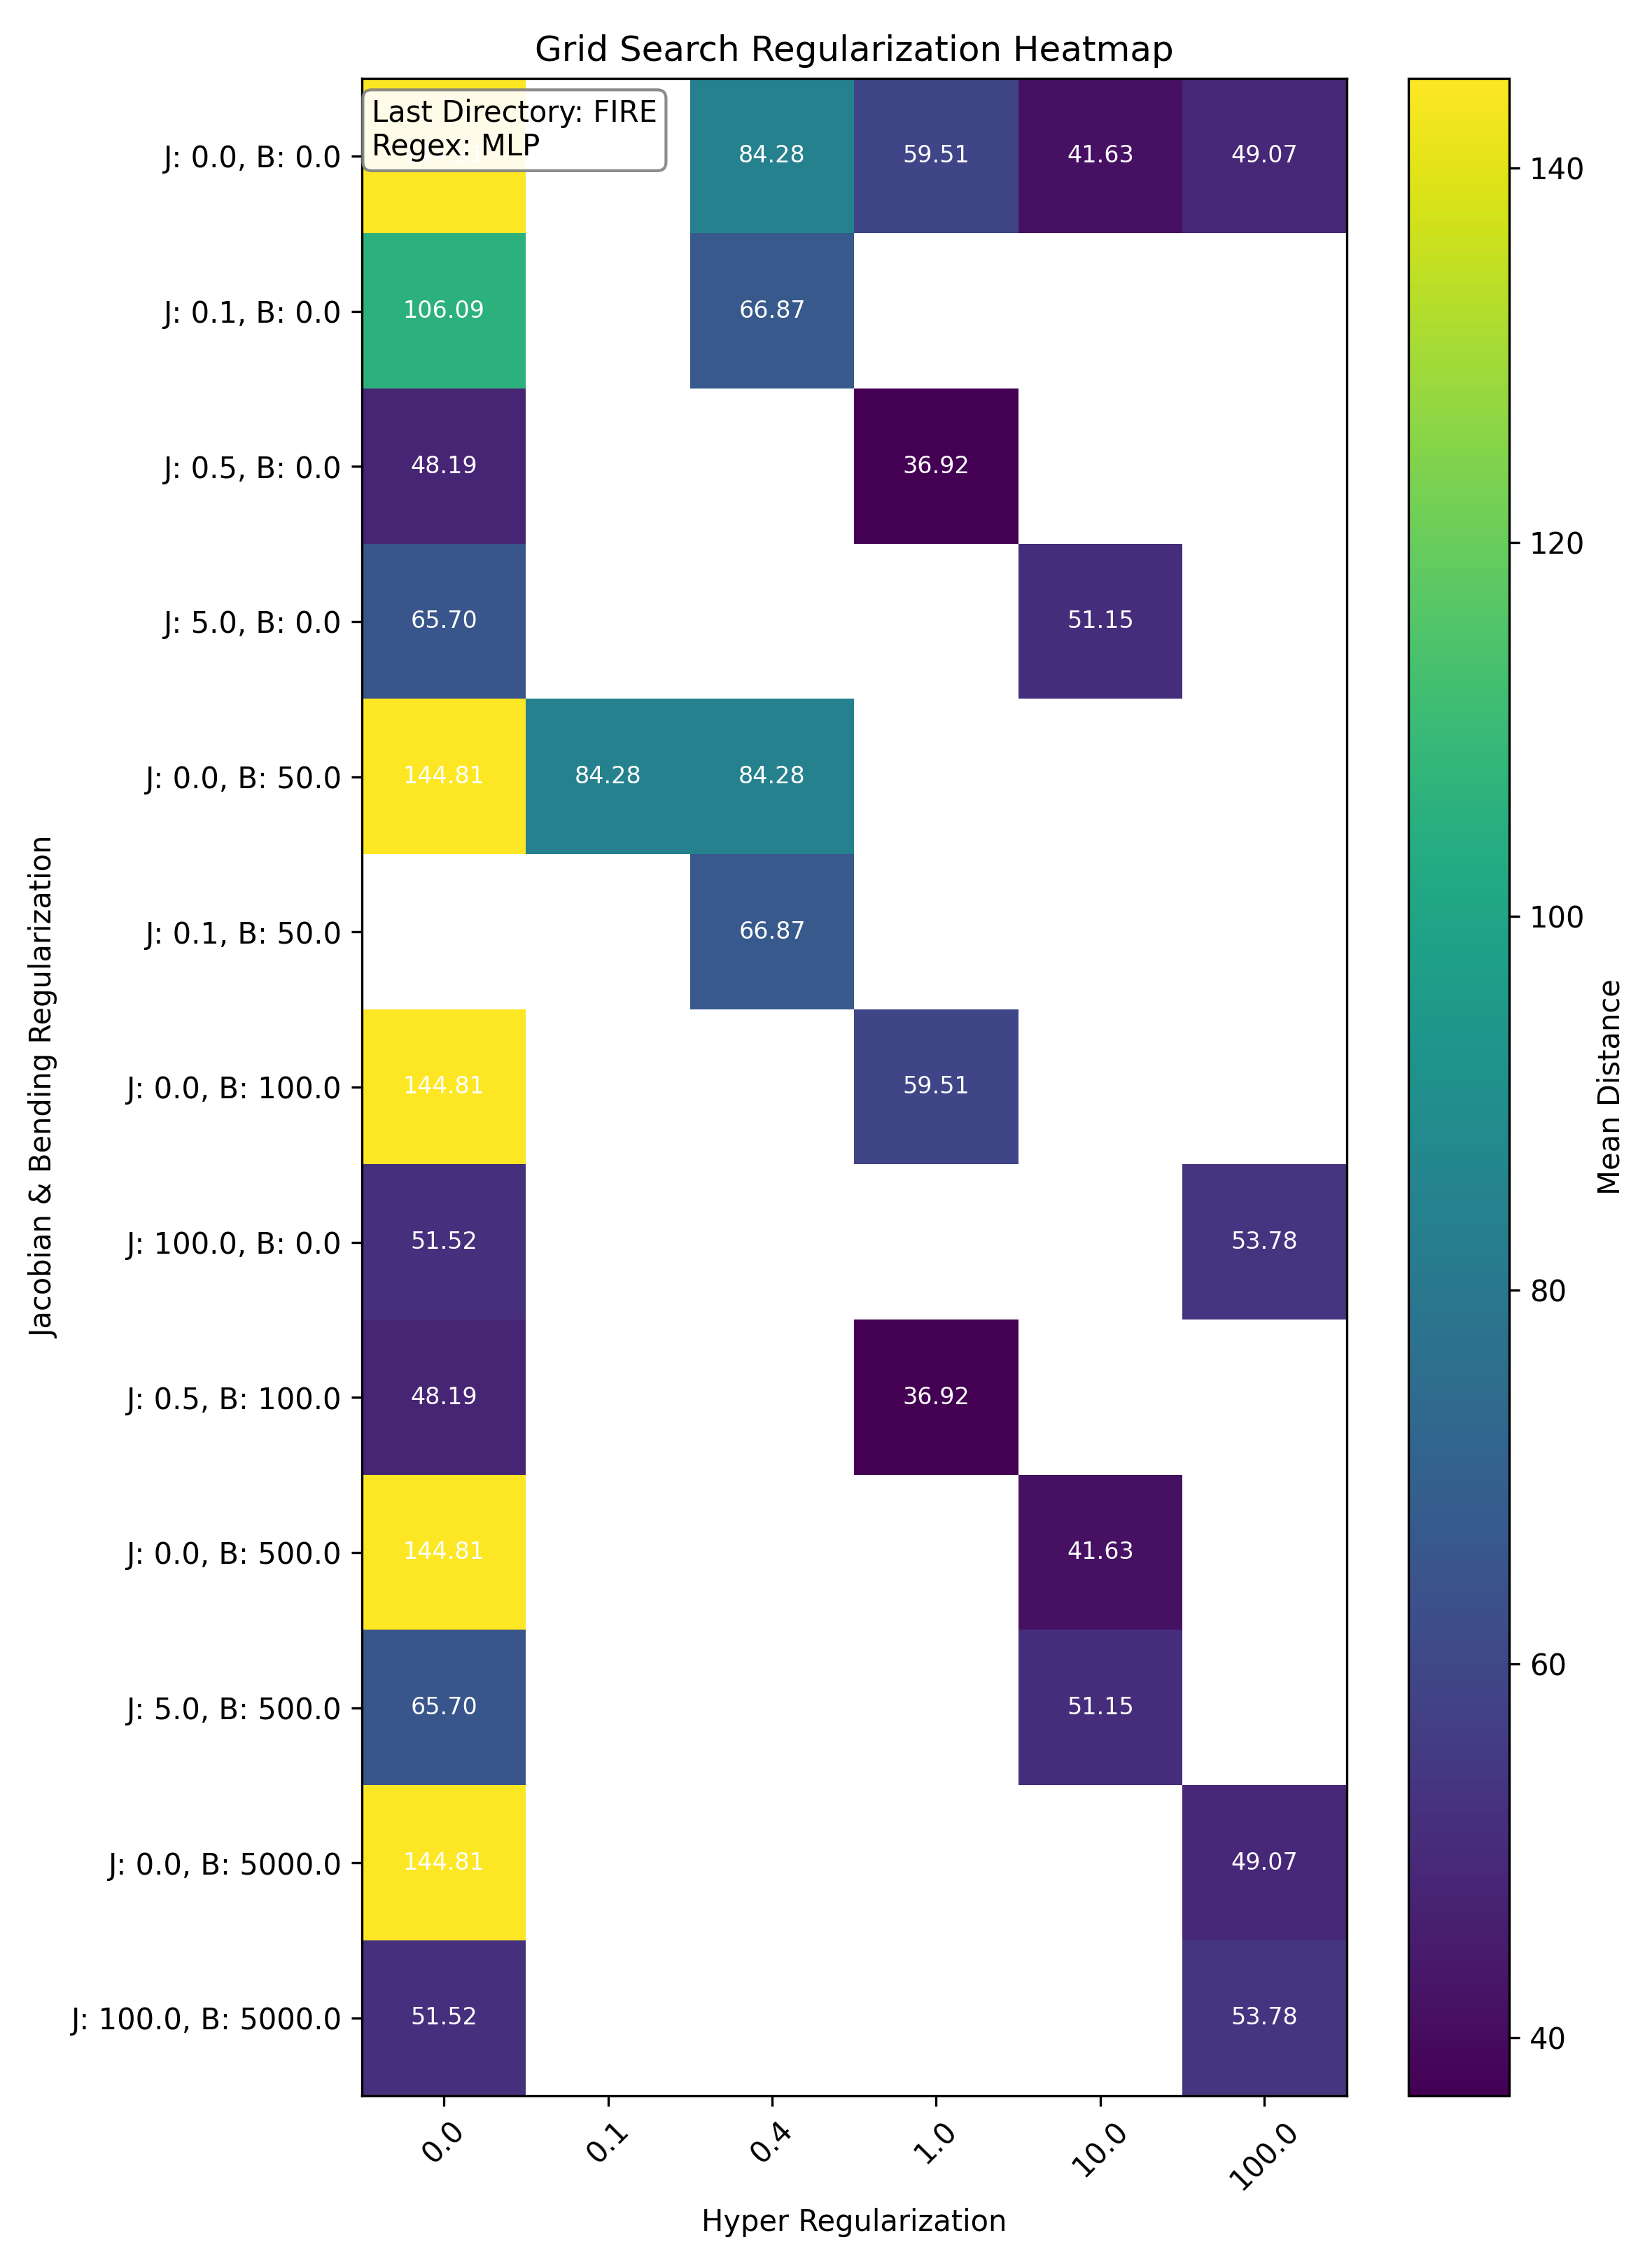
\includegraphics[width=\textwidth]{imaxes/grid_search_single_heatmap_FIRE_MLP.png}
        \caption{FIRE - Relu}
        \label{fig:gs_single_FIRE_MLP}
    \end{subfigure}\hfill
    \begin{subfigure}[b]{0.45\textwidth}
        \centering
        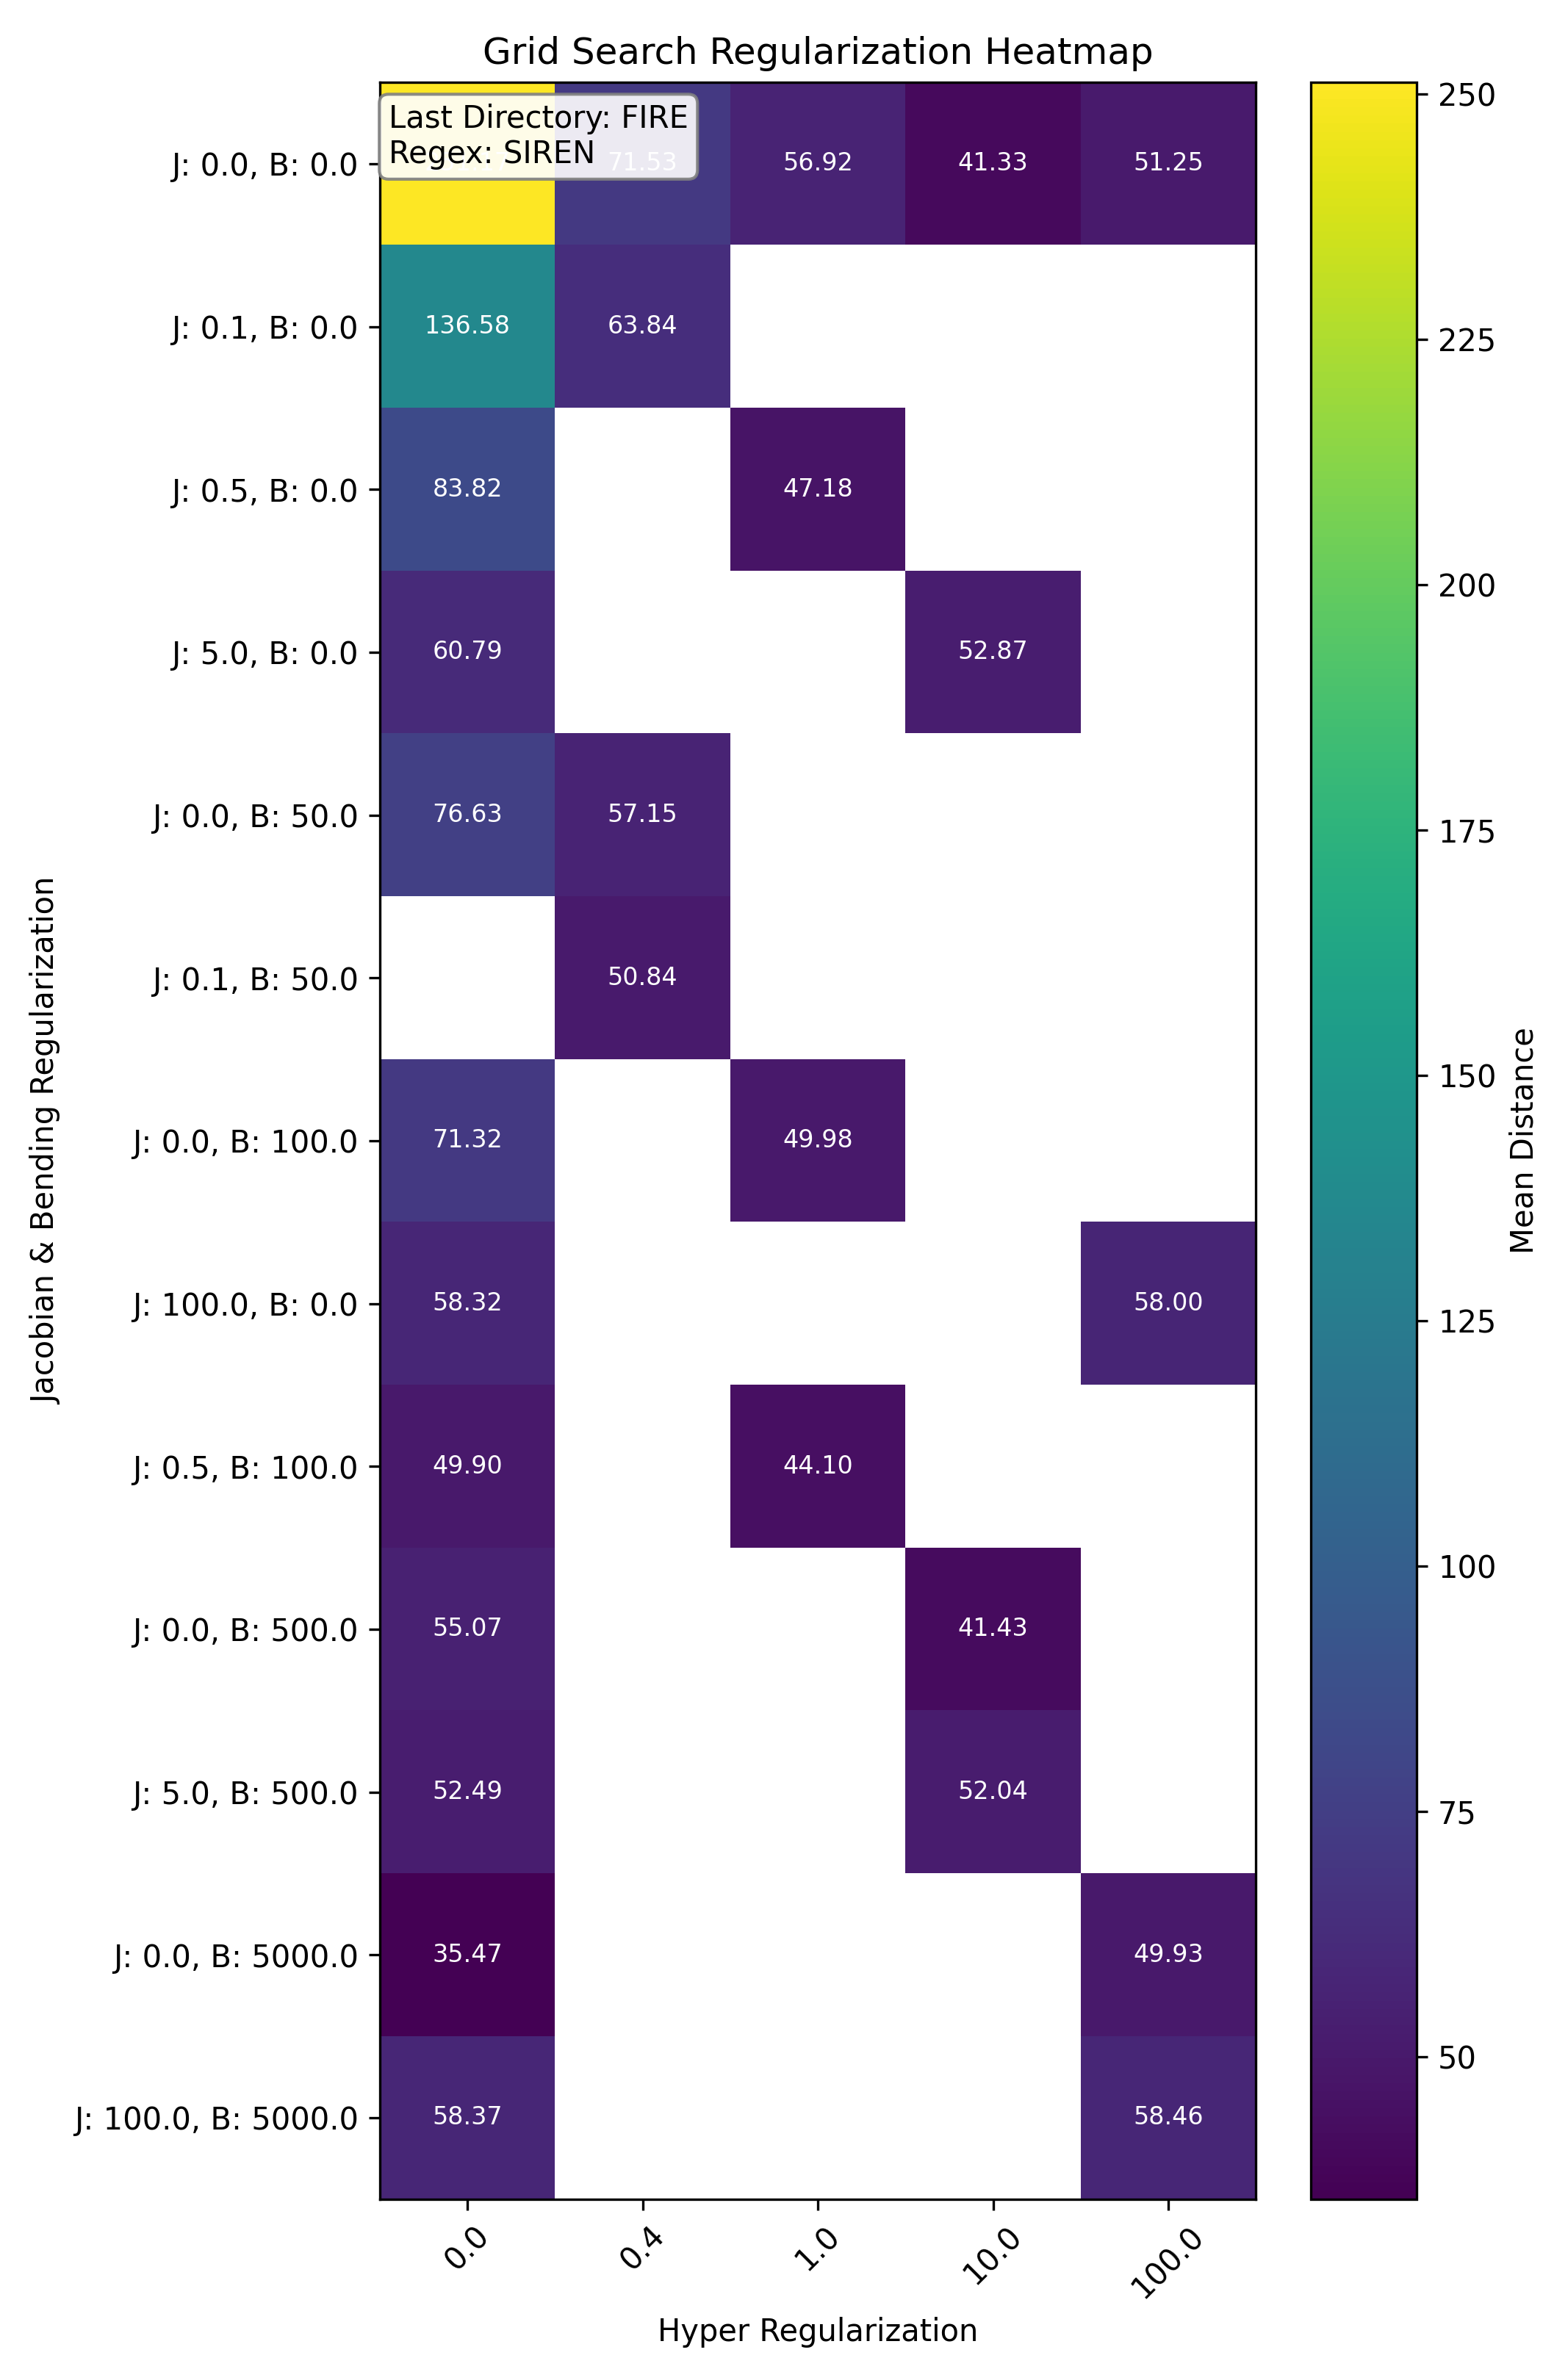
\includegraphics[width=\textwidth]{imaxes/grid_search_single_heatmap_FIRE_SIREN.png}
        \caption{FIRE - SIREN}
        \label{fig:gs_single_FIRE_SIREN}
    \end{subfigure}
    
    \vskip0\baselineskip
    
    \begin{subfigure}[b]{0.45\textwidth}
        \centering
        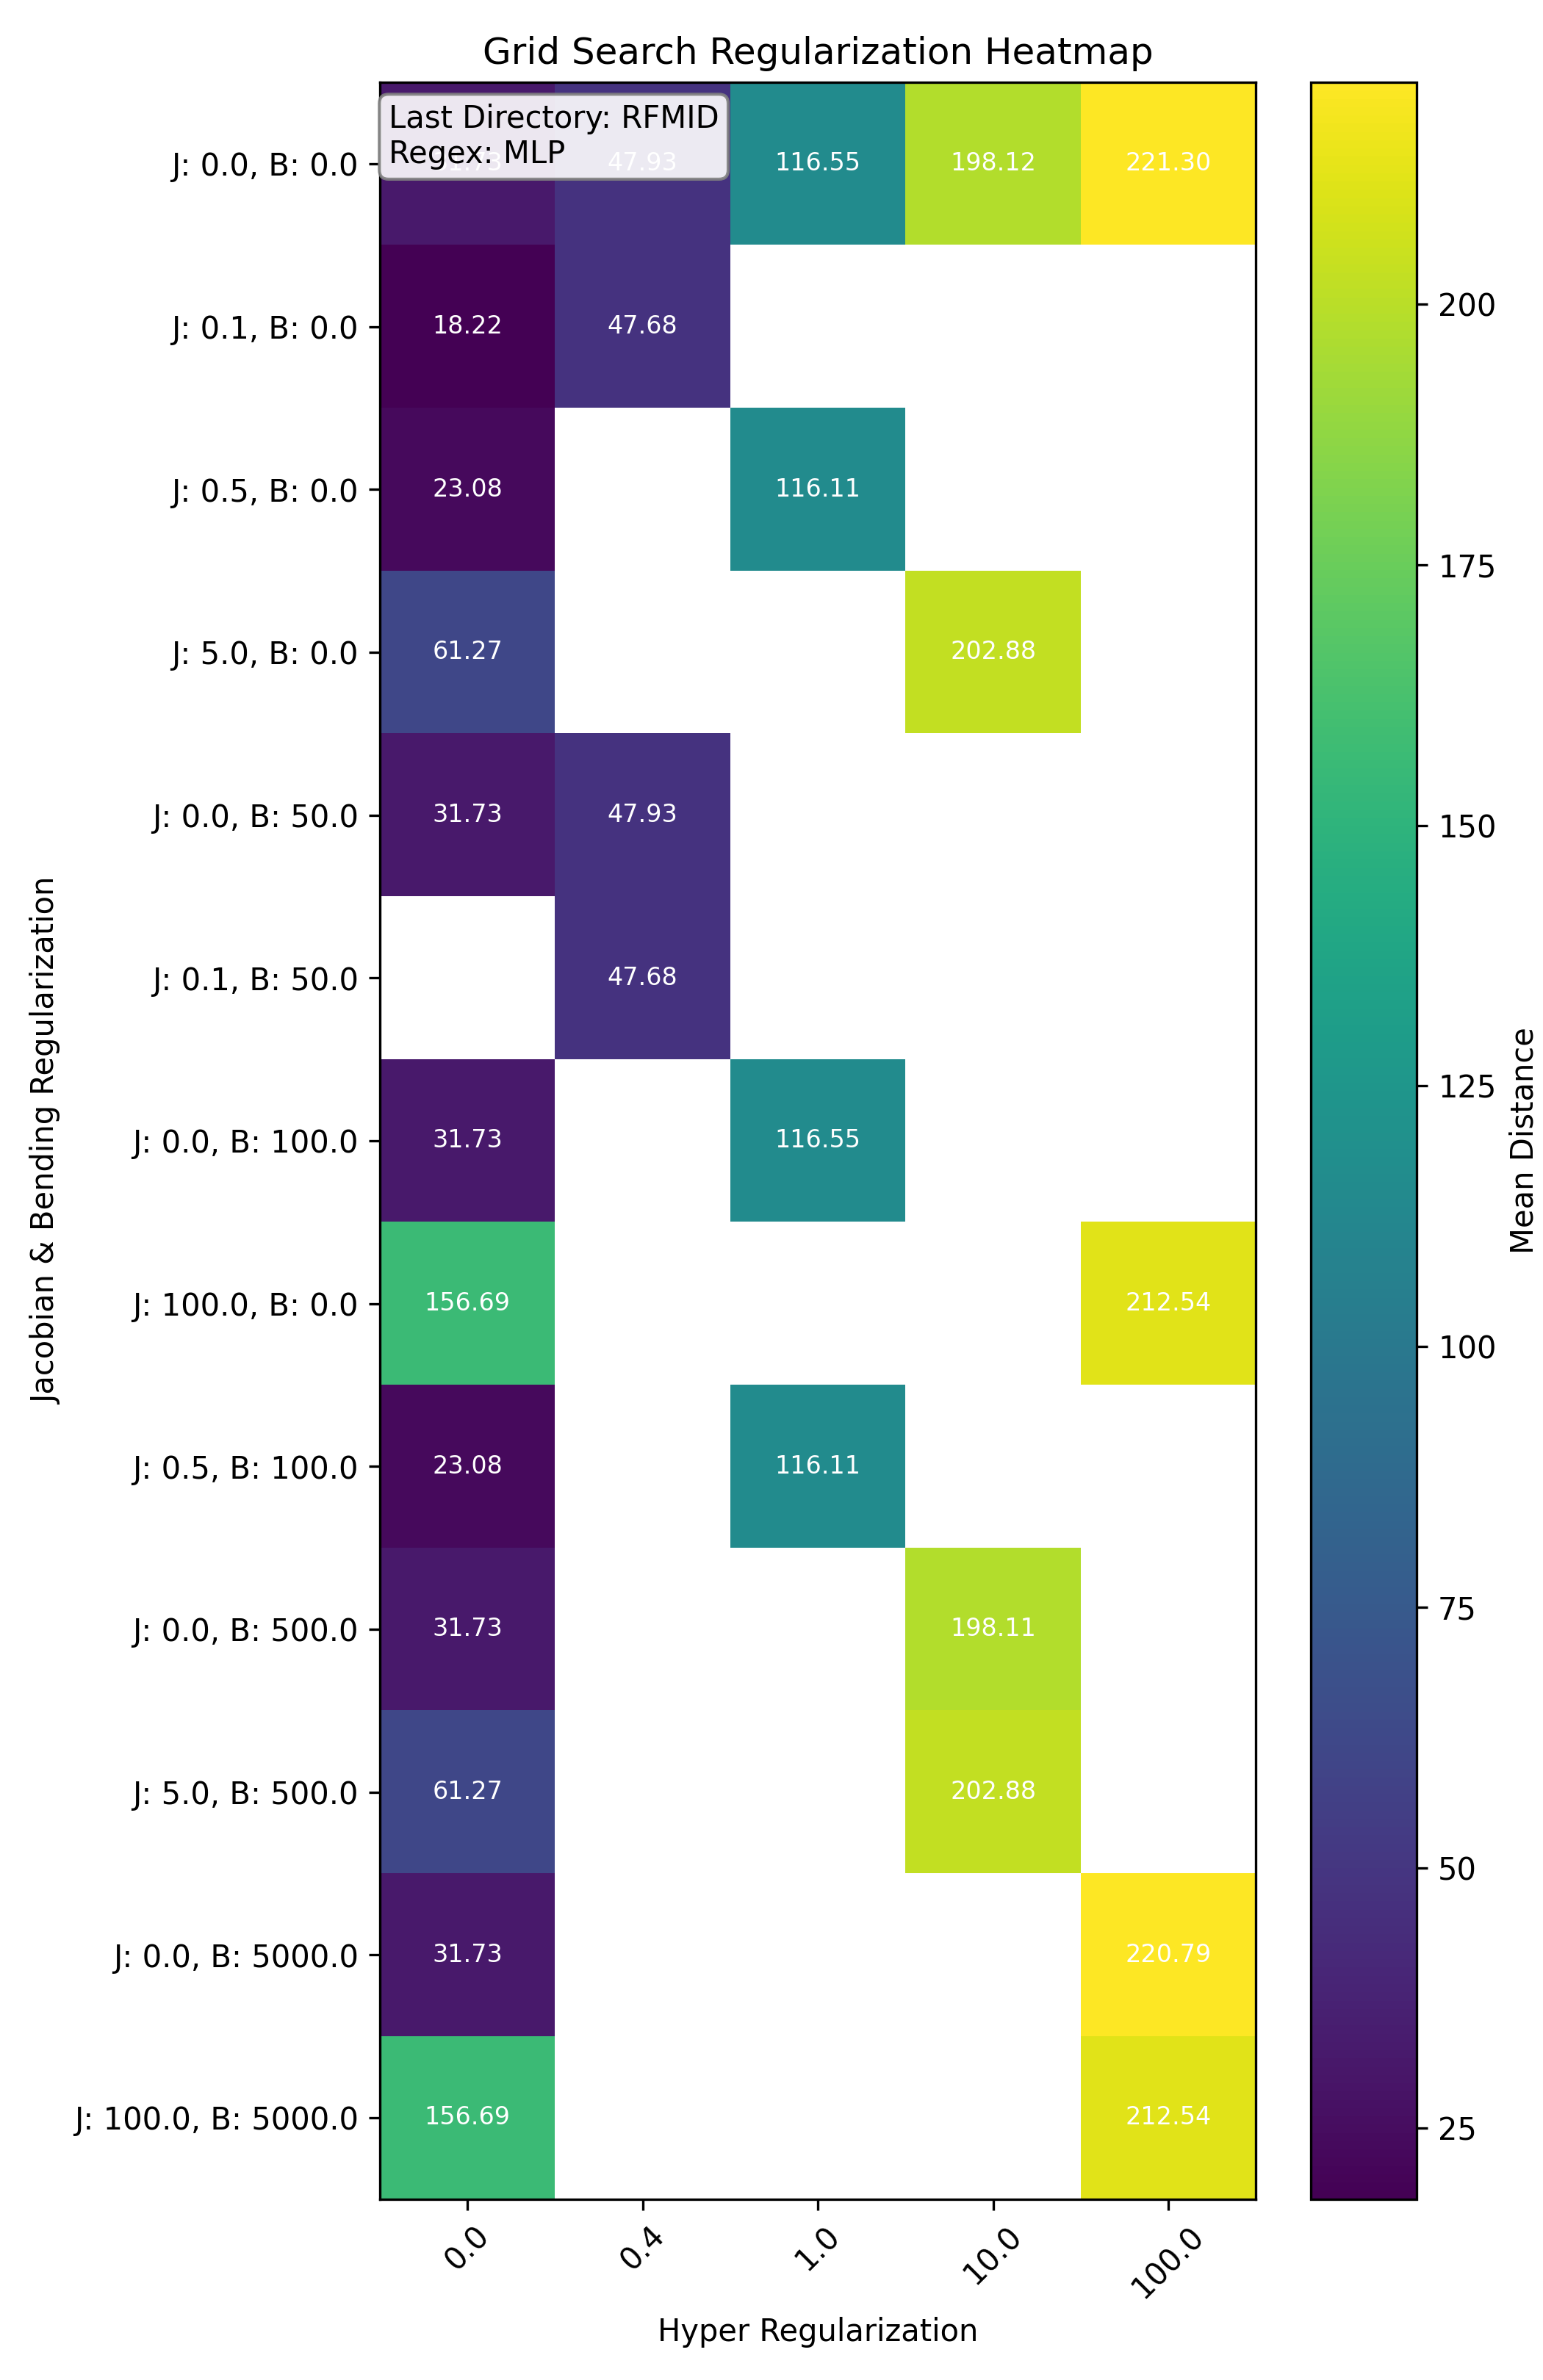
\includegraphics[width=\textwidth]{imaxes/grid_search_single_heatmap_RFMID_MLP.png}
        \caption{RFMID - Relu}
        \label{fig:gs_single_RFMID_MLP}
    \end{subfigure}\hfill
    \begin{subfigure}[b]{0.45\textwidth}
        \centering
        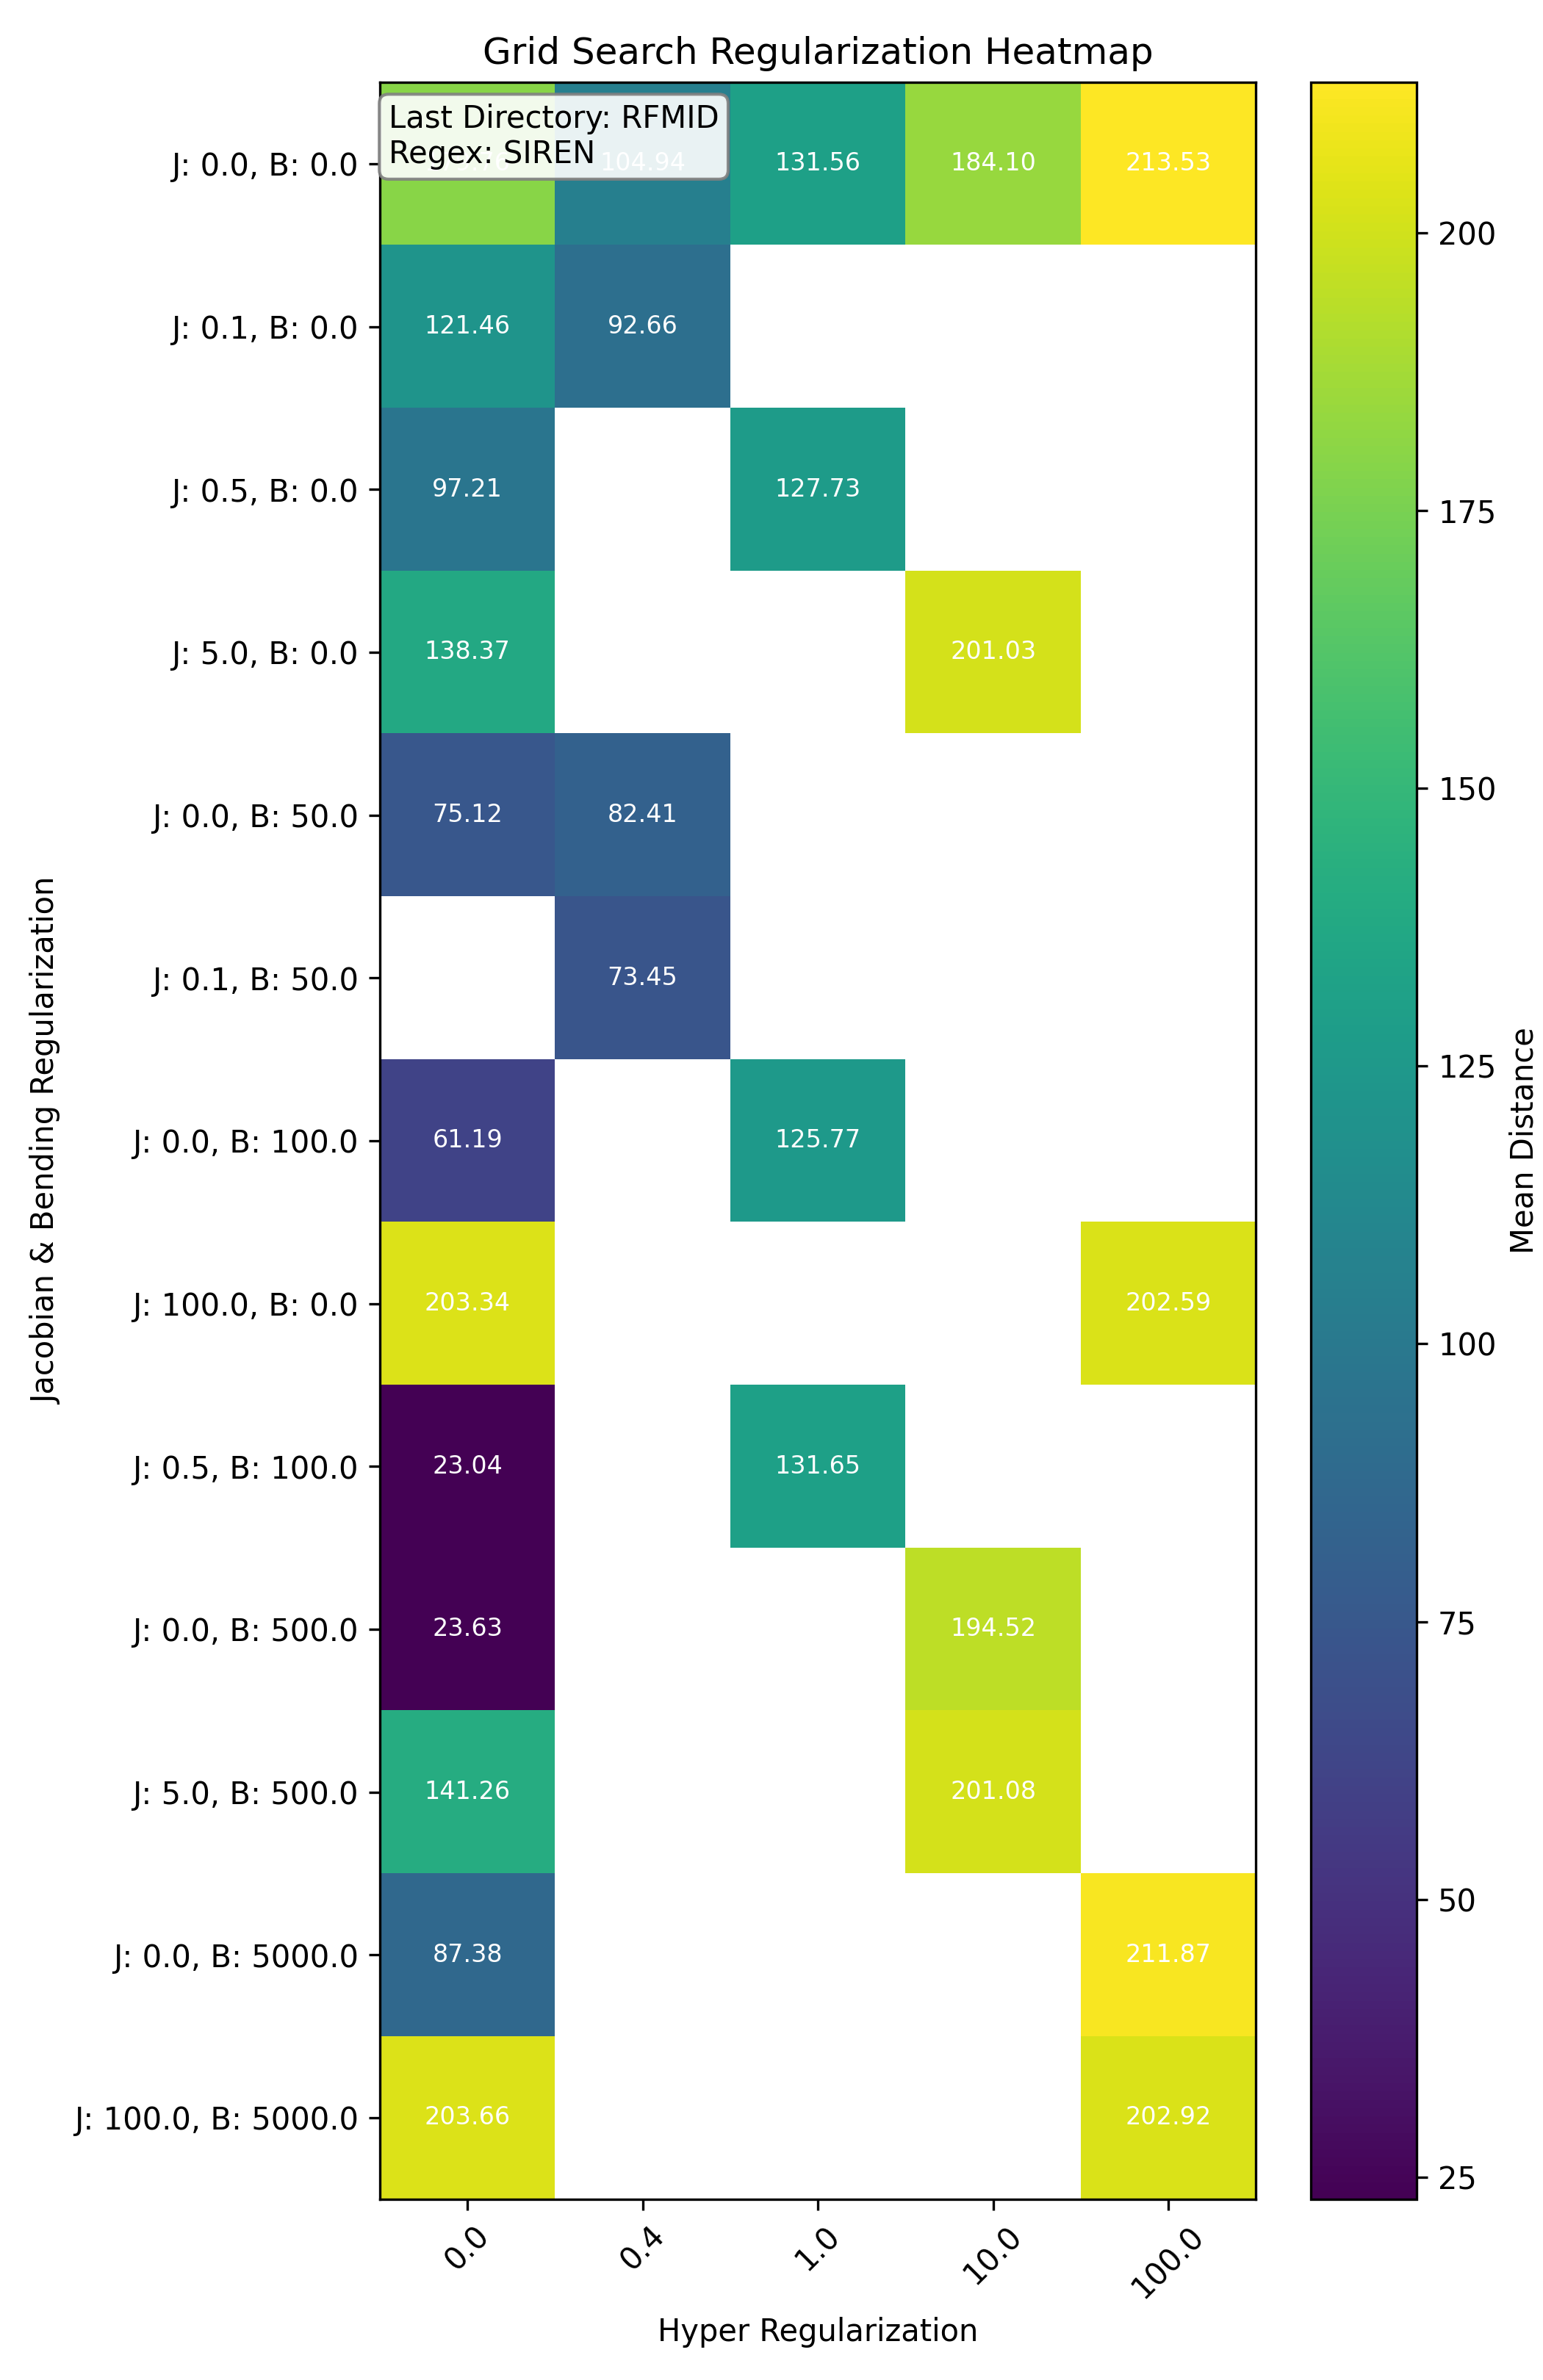
\includegraphics[width=\textwidth]{imaxes/grid_search_single_heatmap_RFMID_SIREN.png}
        \caption{RFMID - SIREN}
        \label{fig:gs_single_RFMID_SIREN}
    \end{subfigure}
    
    \caption{Mapa de calor cos resultados de diferentes combinacións de termos de regularización e funcións de activación sobre os datasets FIRE e RFMID}
    \label{fig:gs_single_heatmaps}
\end{figure}

\paragraph{Discusión}
\label{par:Discusión}

Os resultados amosan que a regularización ten un impacto significativo no rendemento da rede.

\paragraph{Conclusións}
\label{par:Conclusións}

\subsubsection{Learning rate}
\label{subsubsec:Learning rate}

\paragraph{Planteamento}
\label{par:Planteamento}

O learning rate é un parámetro do optimizador (Adam neste caso) que regula o tamaño dos axustes efectuados aos parámetros do modelo durante cada iteración de actualización. Determina a magnitude do cambio aplicado para minimizar a función de perda, afectando tanto a velocidade de converxencia como a estabilidade do proceso de aprendizaxe.
Un learning rate demasiado alto pode provocar que a rede diverxa, mentres que un learning rate demasiado baixo pode resultar en converxencia lenta ou quedar atrapado en mínimos locais.

Debido á natureza da rede, o batch size utilzado ten unha relación directa co learning rate, polo que tentaremos determinar a relación óptima entre ambos.

Unha das heurísiticas mais comúns para relacionar o learning rate e o batch size é a regla de escalado linear \cite{goyal2018accuratelargeminibatchsgd}. 
A regla indica que o learning rate óptimo debe escalarse linearmente co tamaño do batch size. 

Unha forma de explicar isto é, xa que con batches mais grandes temos unha mellor aproximación do gradiente real, é posible utilizar un learning rate maior sen que a rede diverxa.

Para determinar cal é o learning rate óptimo, realizáronse experimentos comparando o rendemento de cada un sobre unha mostra de imaxes dos datases de FIRE e RFMID cas diferentes funcións de activación.

\paragraph{Resultados}
\label{par:Resultados}

\ref{fig:grid_search_lr}, \ref{fig:e_heatmap_MLP_RFMID}

\begin{figure}[ht]
    \centering
    \begin{subfigure}[b]{0.45\textwidth}
        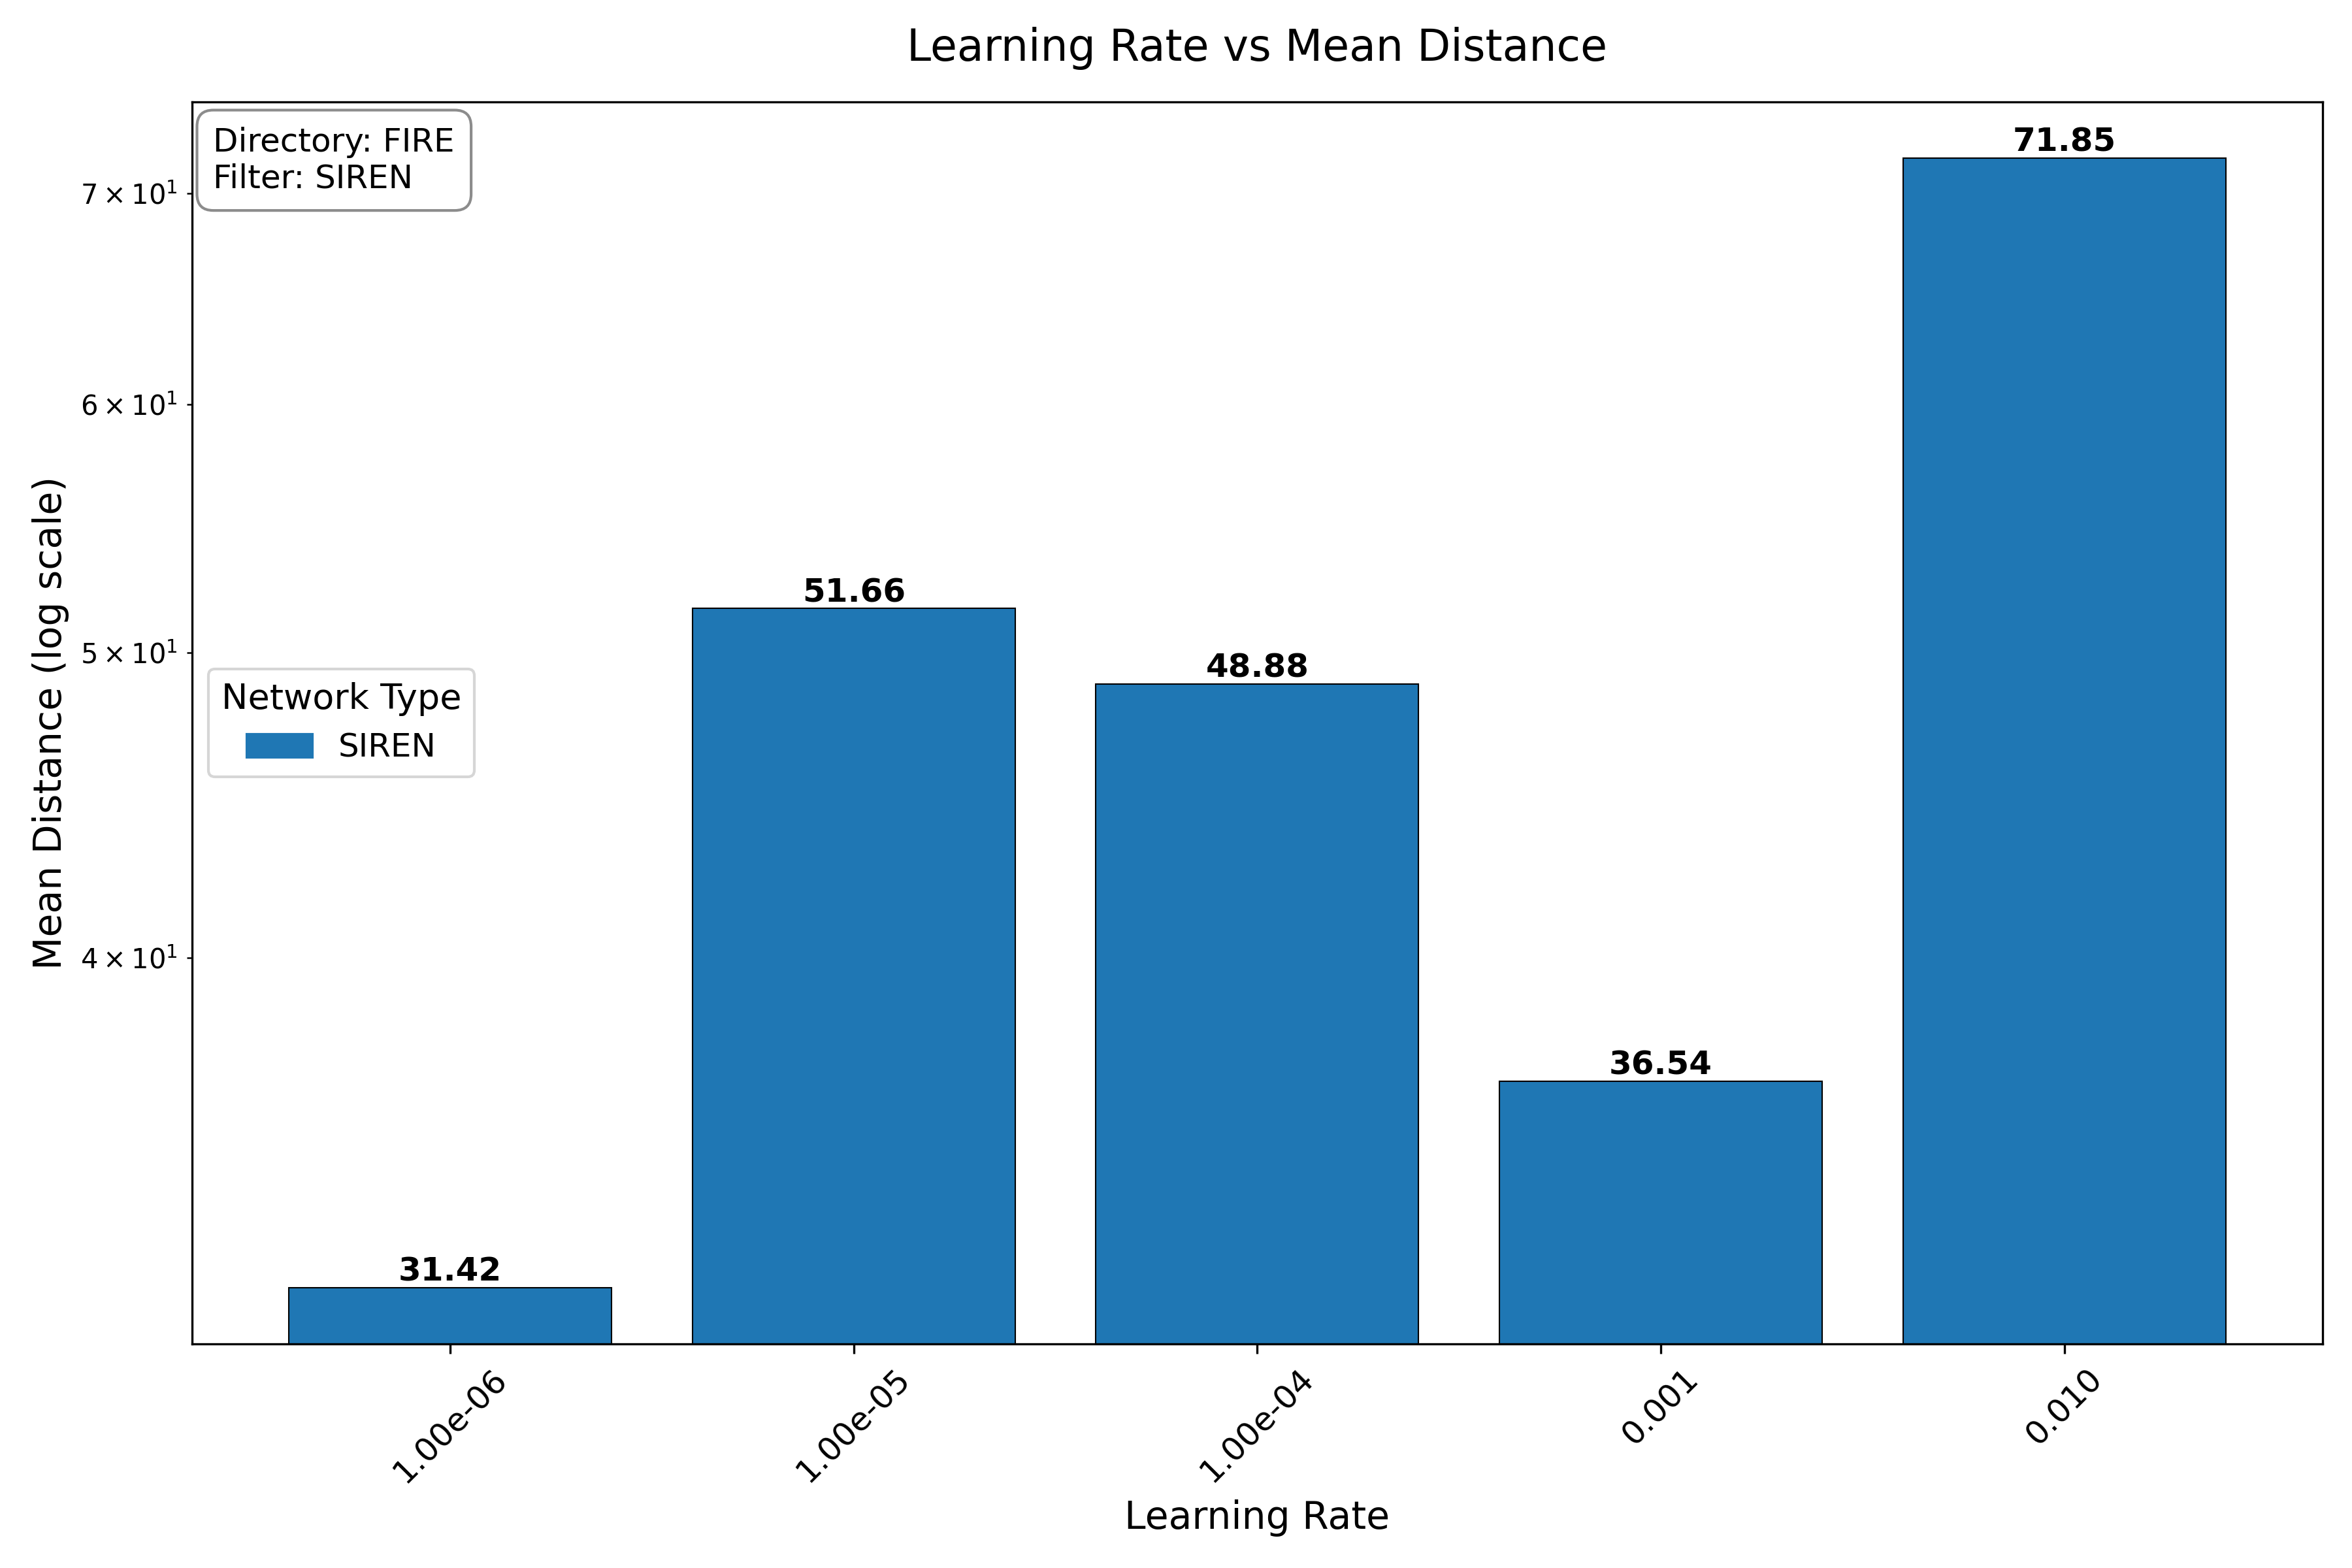
\includegraphics[width=\textwidth]{imaxes/grid_search_lr_FIRE_SIREN.png}
        \caption{FIRE - SIREN}
        \label{fig:grid_search_lr_FIRE_SIREN}
    \end{subfigure}\hfill
    \begin{subfigure}[b]{0.45\textwidth}
        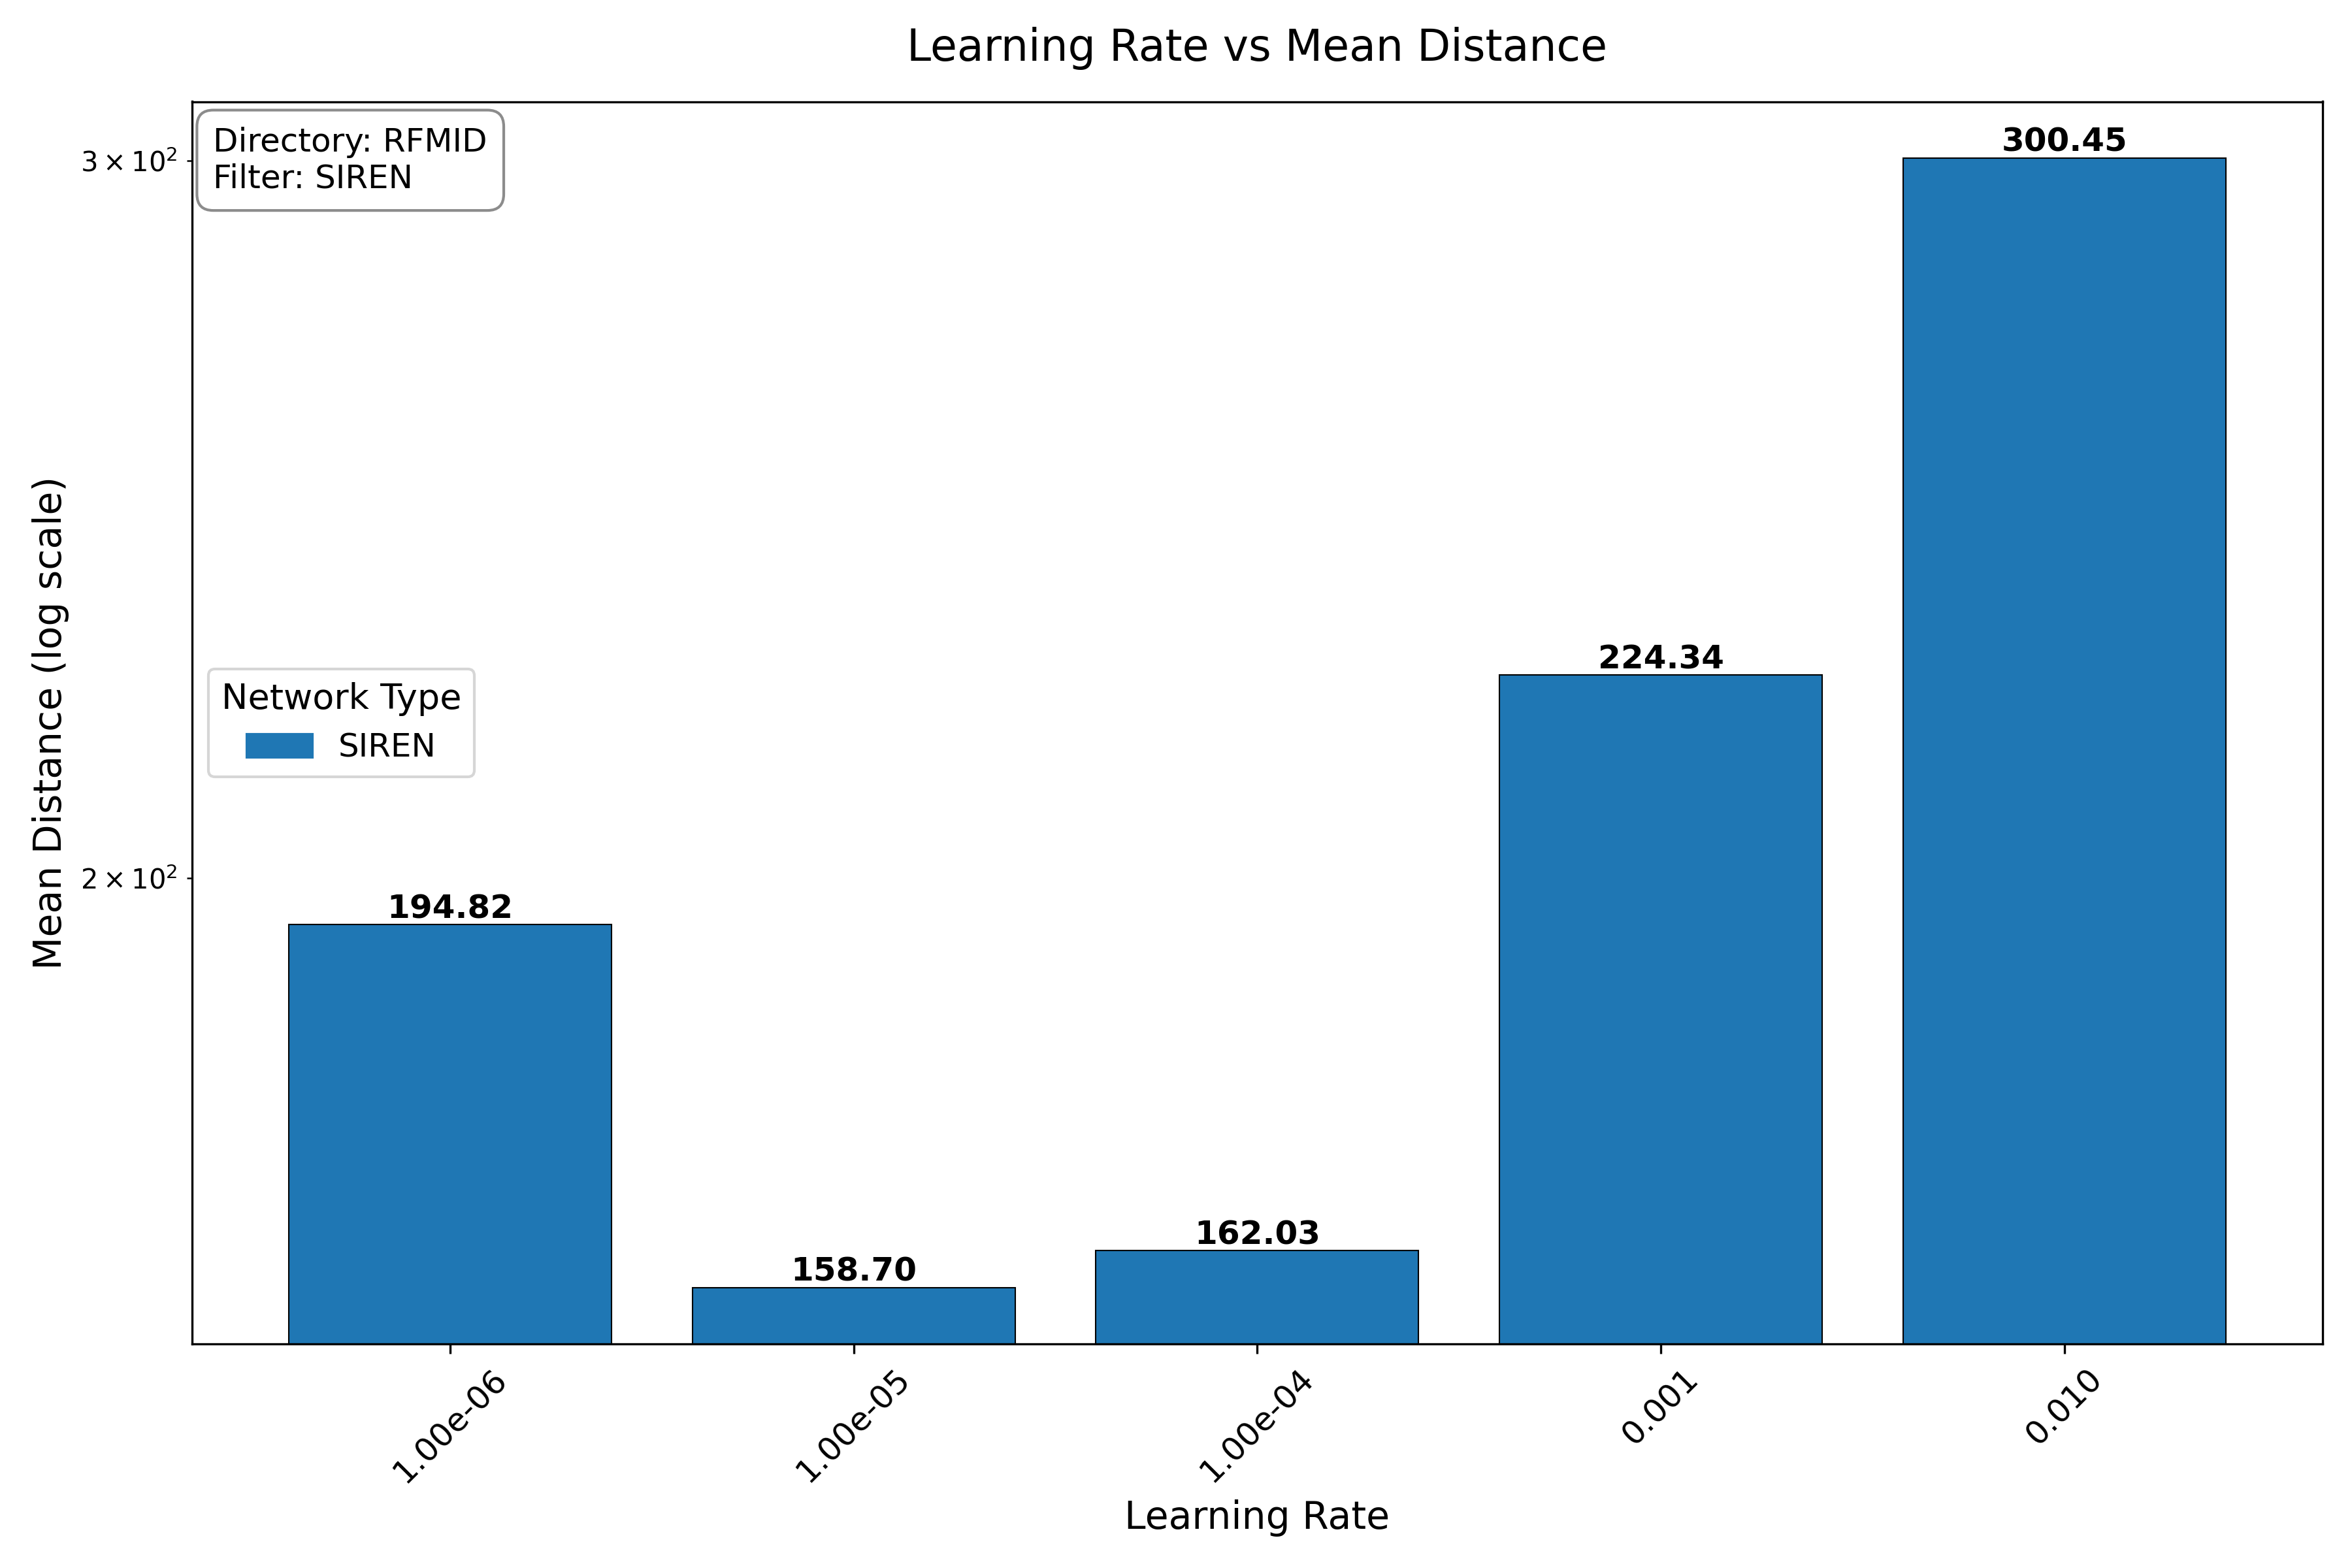
\includegraphics[width=\textwidth]{imaxes/grid_search_lr_RFMID_SIREN.png}
        \caption{RFMID - SIREN}
        \label{fig:grid_search_lr_RFMID_SIREN}
    \end{subfigure}
    \vskip\baselineskip
    \begin{subfigure}[b]{0.45\textwidth}
        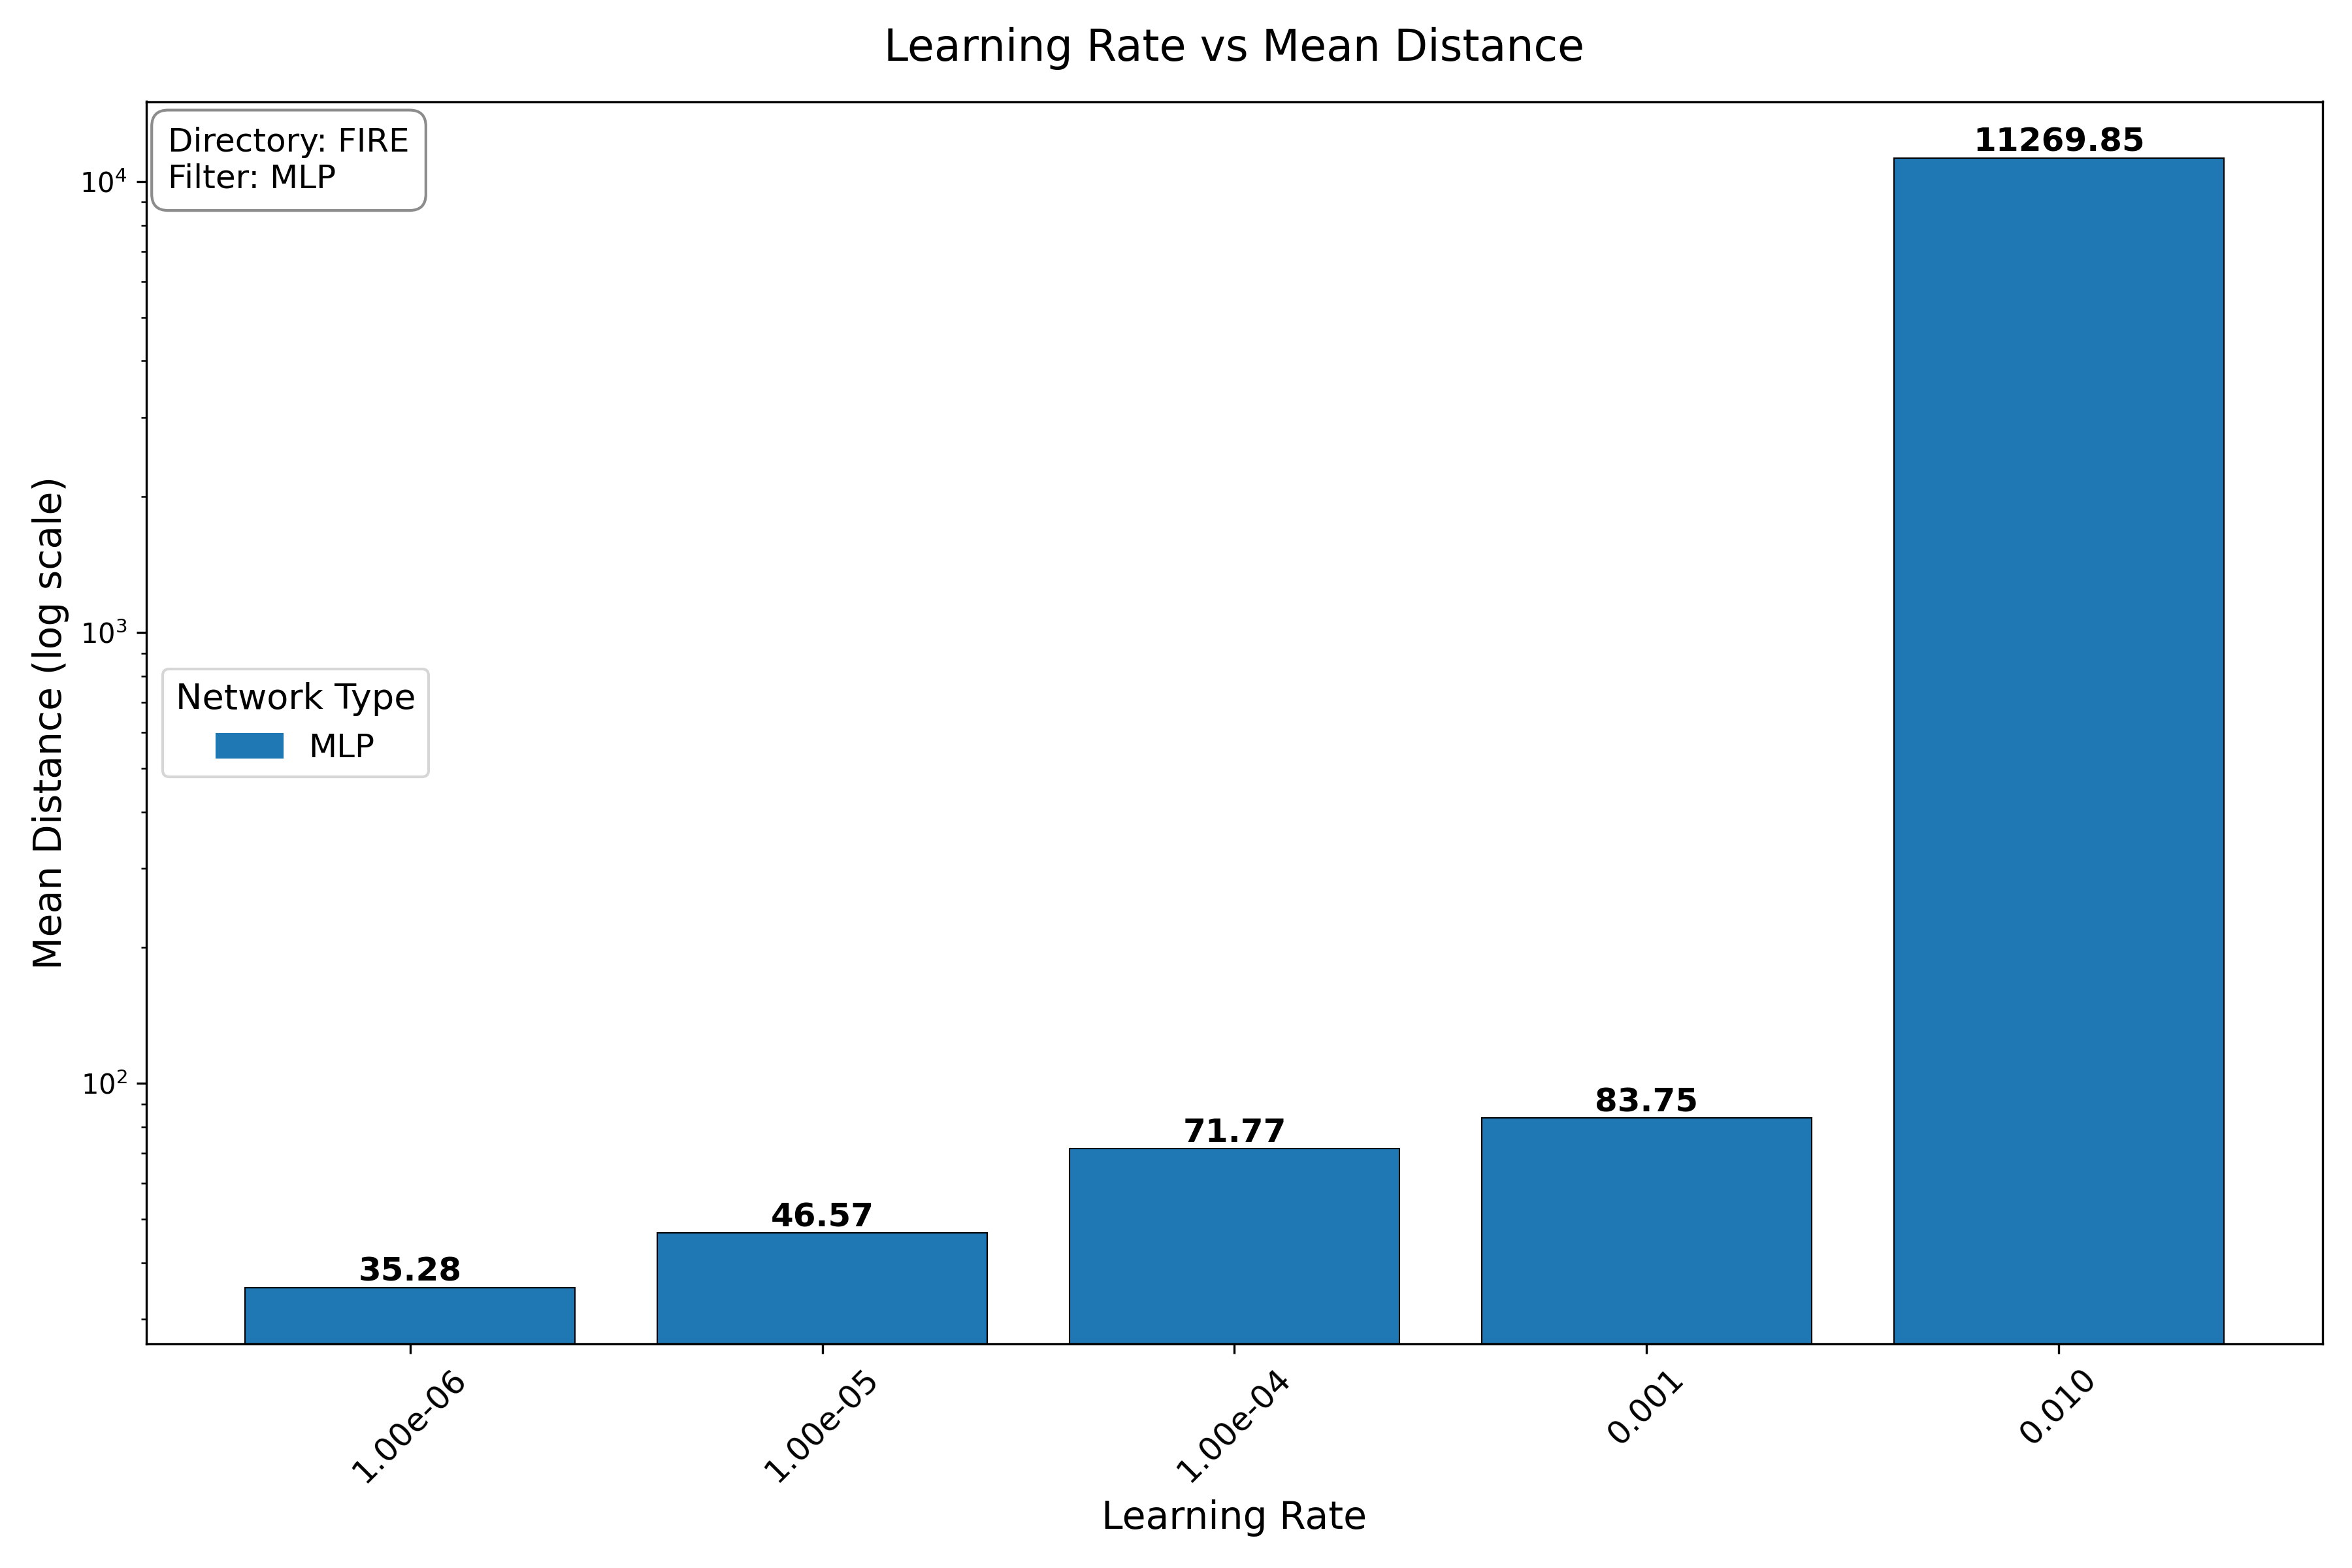
\includegraphics[width=\textwidth]{imaxes/grid_search_lr_FIRE_MLP.png}
        \caption{FIRE - Relu}
        \label{fig:grid_search_lr_FIRE_MLP}
    \end{subfigure}\hfill
    \begin{subfigure}[b]{0.45\textwidth}
        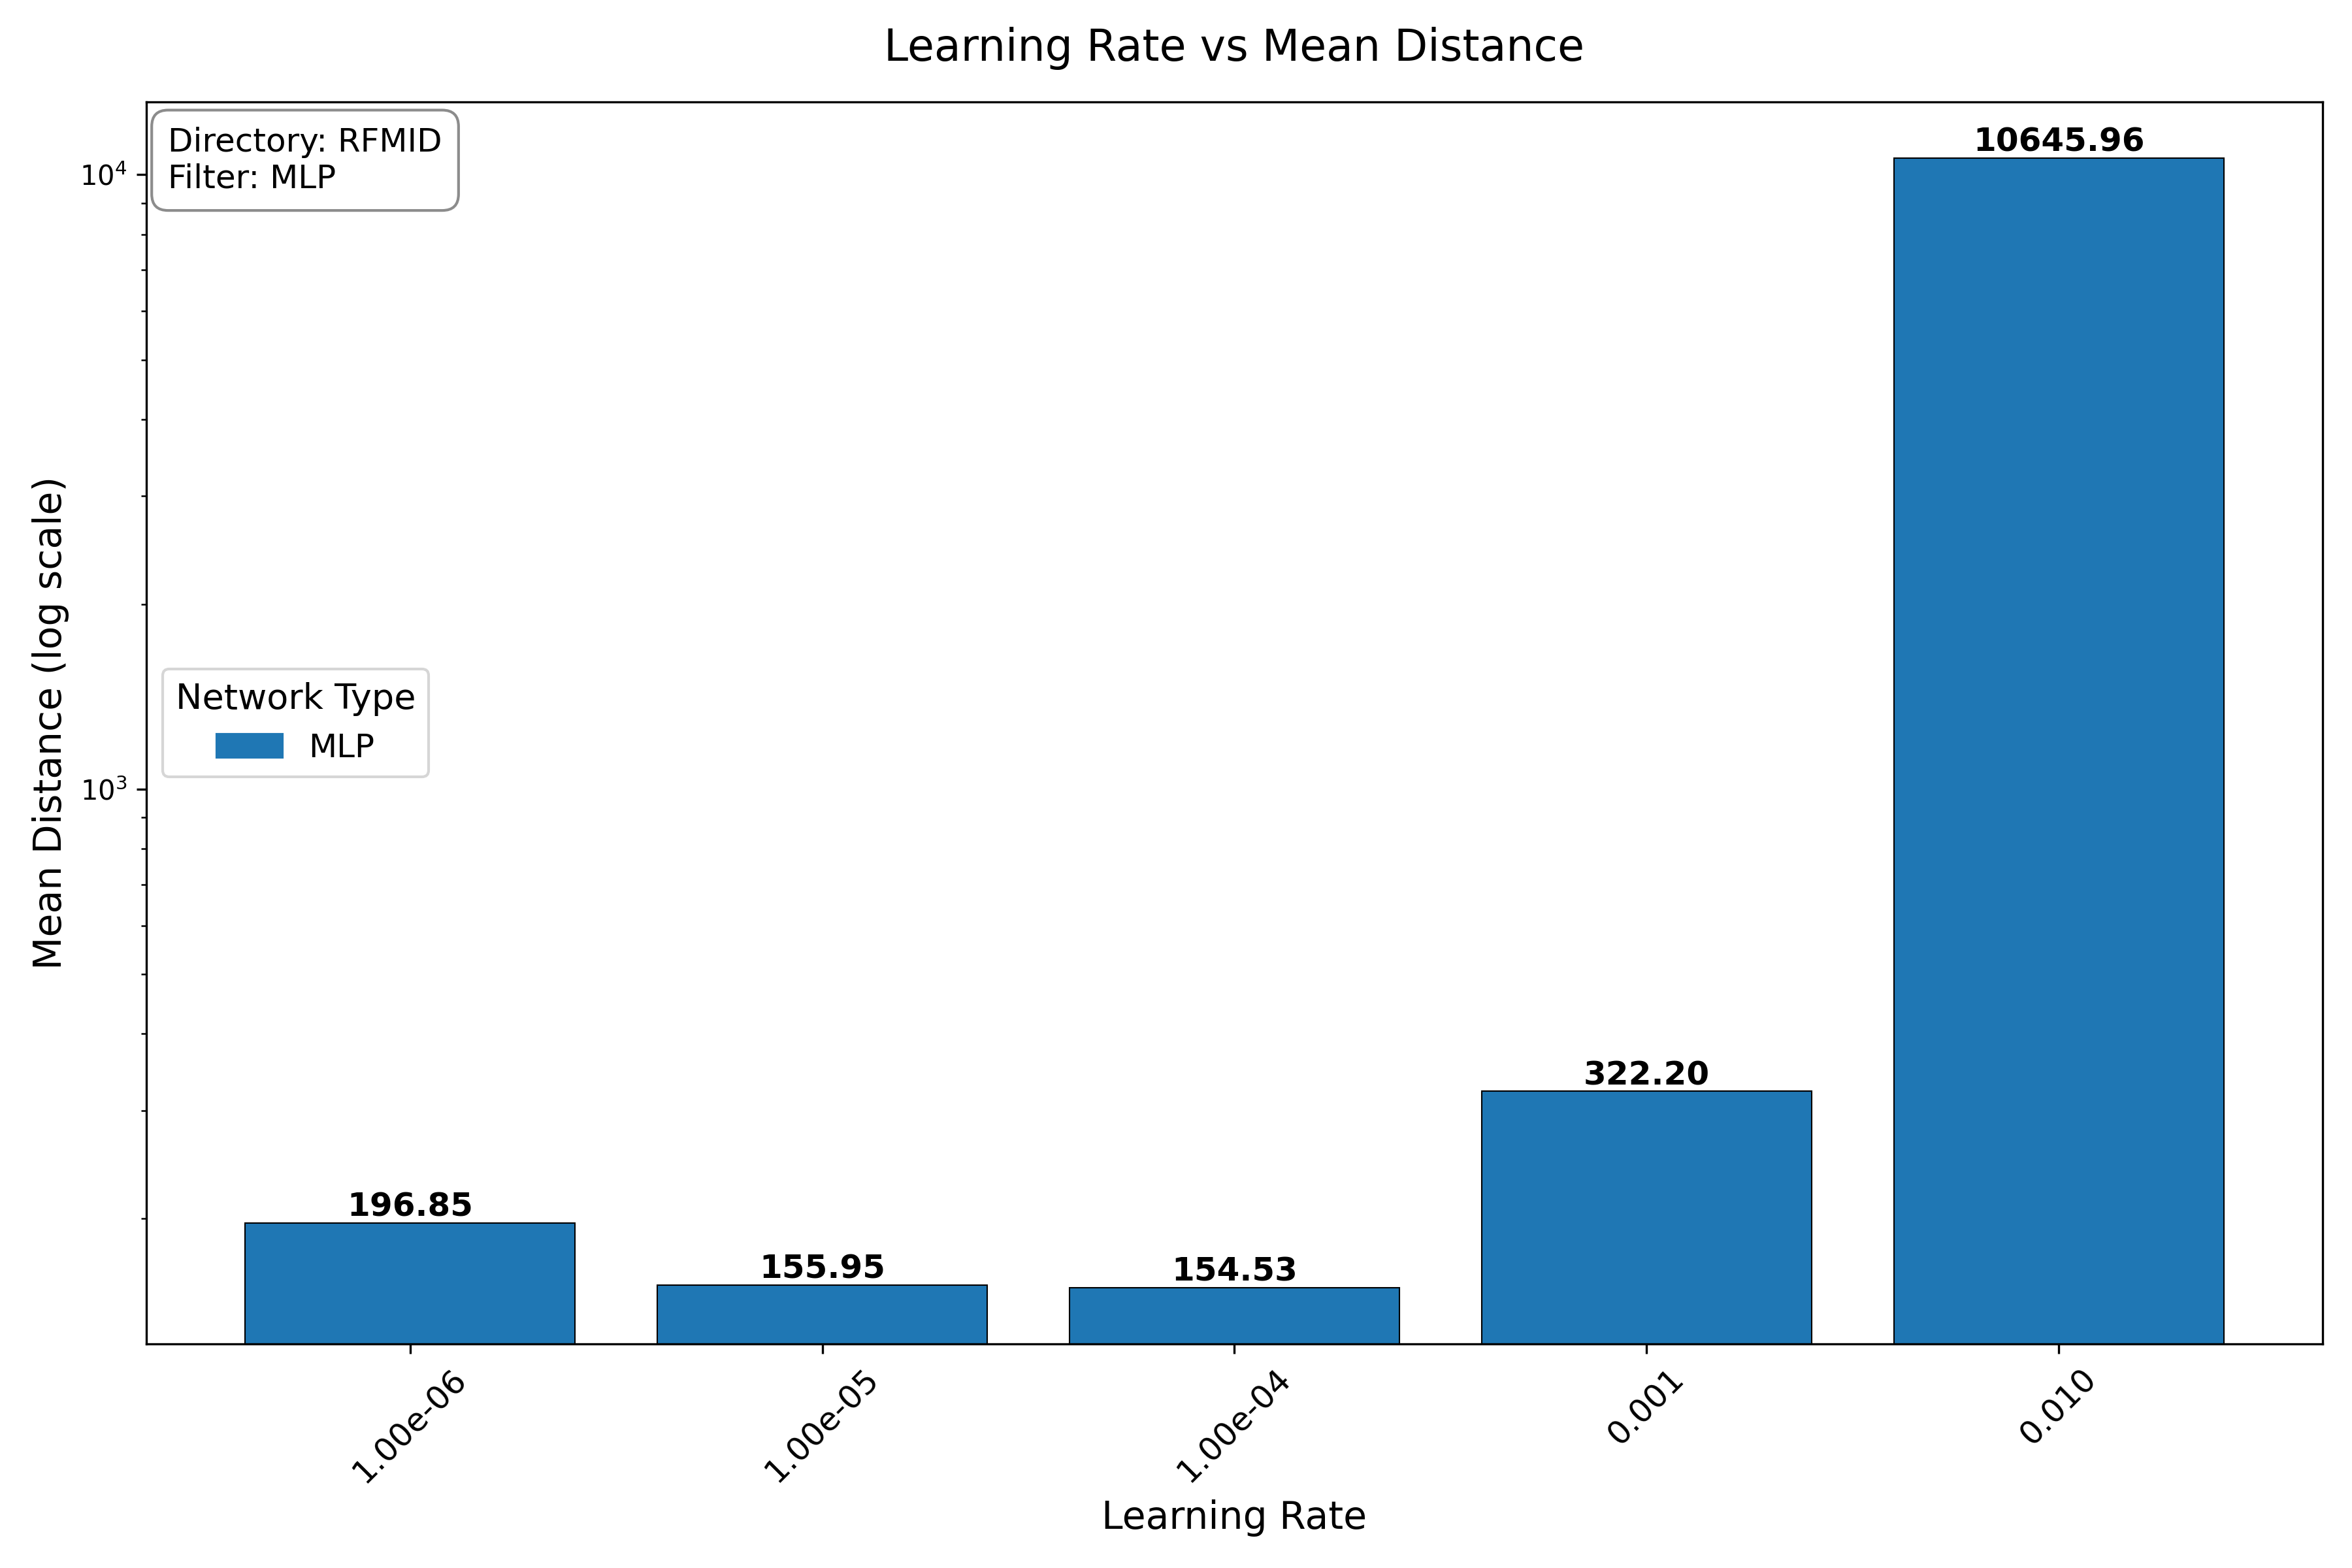
\includegraphics[width=\textwidth]{imaxes/grid_search_lr_RFMID_MLP.png}
        \caption{RFMID - Relu}
        \label{fig:grid_search_lr_RFMID_MLP}
    \end{subfigure}
    \caption{Reusltados lr cos datasets FIRE e RFMID cas funcións de activación SIREN e Relu.}
    \label{fig:grid_search_lr}
\end{figure}

\begin{figure}[ht]
    \centering
    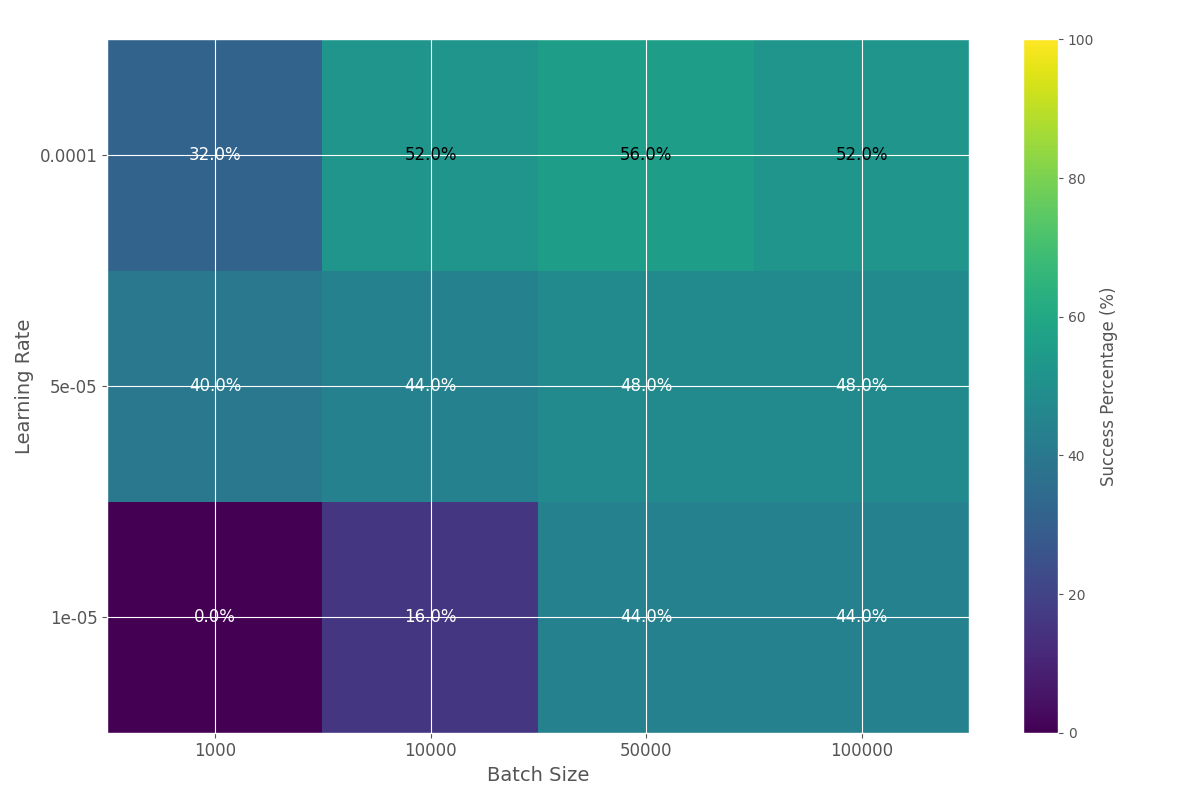
\includegraphics[width=0.8\textwidth]{imaxes/e_heatmap_MLP_RFMID.png}
    \caption{Mapa de calor cos resultados de diferentes combinacións de batch size e learning rate con unha mostra de imaxes de RMIFD ca función de activación ReLU}
    \label{fig:e_heatmap_MLP_RFMID}
\end{figure}

\paragraph{Discusión}
\label{par:Discusión}

Valores de learning rate moi altos (0.001 and 0.005) son contraproducentes, xa que a rede diverxe rapidamente.

A dependencia entre o learning rate e o batch size confirmase. Xeralmente un learning rate baixo (1.0e-05, 1.0e-06) parece requerir de batch sizes maiores e viceversa, o cal é consistente co que se esperaba.

Tamén observase que batch sizes maiores tenden a dar mellores resultados.

\paragraph{Conclusións}
\label{par:Conclusións}

\subsection{Batch size}
\label{subsec:Batch size}

\paragraph{Planteamento}
\label{par:Planteamento}

Ao longo dos experimentos realizados, o análisis cualitativo revelou que o batch size é un dos parámetros que máis impacto ten no rendemento da rede.
Unha vez determinados uns valores aceptables nos parámetros anteriores, realizáronse experimentos para determinar cal era o batch size óptimo.

Neste caso dividimos o conxunto de datos de RFMID en varios subconxuntos según a dificultade da transformación, medida mediante a norma de Frobenius.
A norma de Frobenius dunha matriz $A \in \mathbb{R}^{m \times n}$ defínese como:

\[
\|A\|_F = \sqrt{\sum_{i=1}^{m} \sum_{j=1}^{n} |a_{ij}|^2}
\]

onde $a_{ij}$ son os elementos da matriz $A$.
Esta é unha xeralización da distancia euclidiana aplicada a matrices, onde as imaxes con transformacións mais grandes considéranse mais difíciles.

Desta forma podemos comparar o rendemento da rede en diferentes subconxuntos de imaxes, e determinar se o rendemento da rede é consistente entre eles.
Ademais, xa que a rede si que é capaz de rexistrar correctamente as imaxes dos subconxuntos mais sinxelos, utilizaremos a métrica de FIRE para medir o pocentaxe de imaxes rexistradas correctamente.

\paragraph{Resultados}
\label{par:Resultados}

\ref{fig:batch_size_comparison_relu_1e-5}, \ref{fig:batch_size_comparison_relu_5e-5}, \ref{fig:batch_size_comparison_relu_1e-4}
\ref{fig:batch_size_comparison_siren_1e-4}, \ref{fig:batch_size_comparison_siren_1e-5}, \ref{fig:batch_size_comparison_siren_5e-5}

\begin{figure}[ht] 
    \centering
    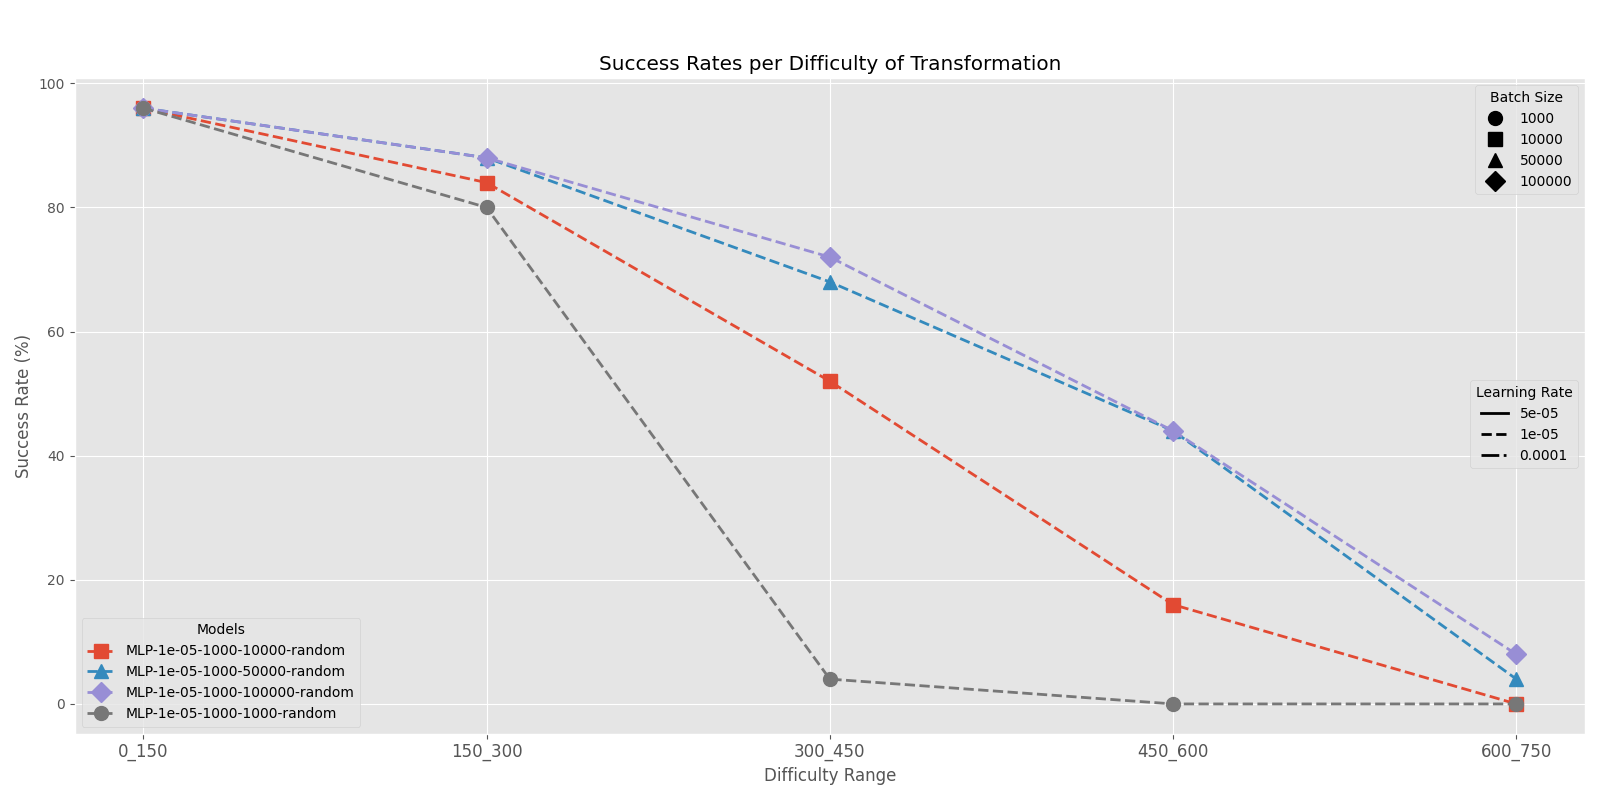
\includegraphics[width=0.8\textwidth]{imaxes/batchsize/experiment_plot_RFMID_MLP_1e-05.png}
    \caption{Comparación do rendemento da rede con diferentes batch sizes sobre imaxes do dataset RFMID ca función de activación ReLU (learning rate = 1e-5)}
    \label{fig:batch_size_comparison_relu_1e-5}
\end{figure}

\begin{figure}[ht] 
    \centering
    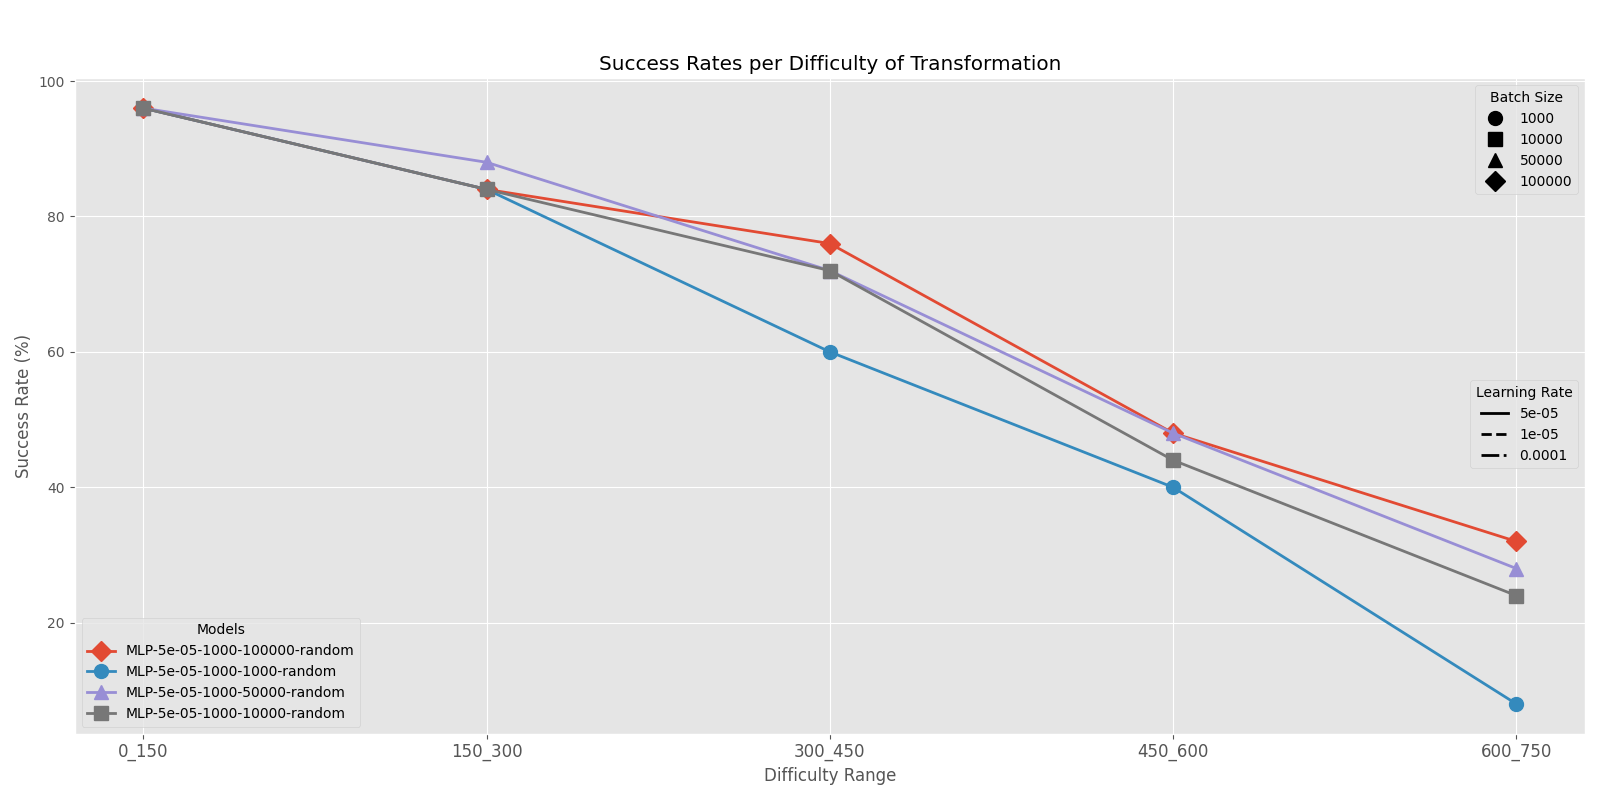
\includegraphics[width=0.8\textwidth]{imaxes/batchsize/experiment_plot_RFMID_MLP_5e-05.png}
    \caption{Comparación do rendemento da rede con diferentes batch sizes sobre imaxes do dataset RFMID ca función de activación ReLU (learning rate = 5e-5)}
    \label{fig:batch_size_comparison_relu_5e-5}
\end{figure}

\begin{figure}[ht] 
    \centering
    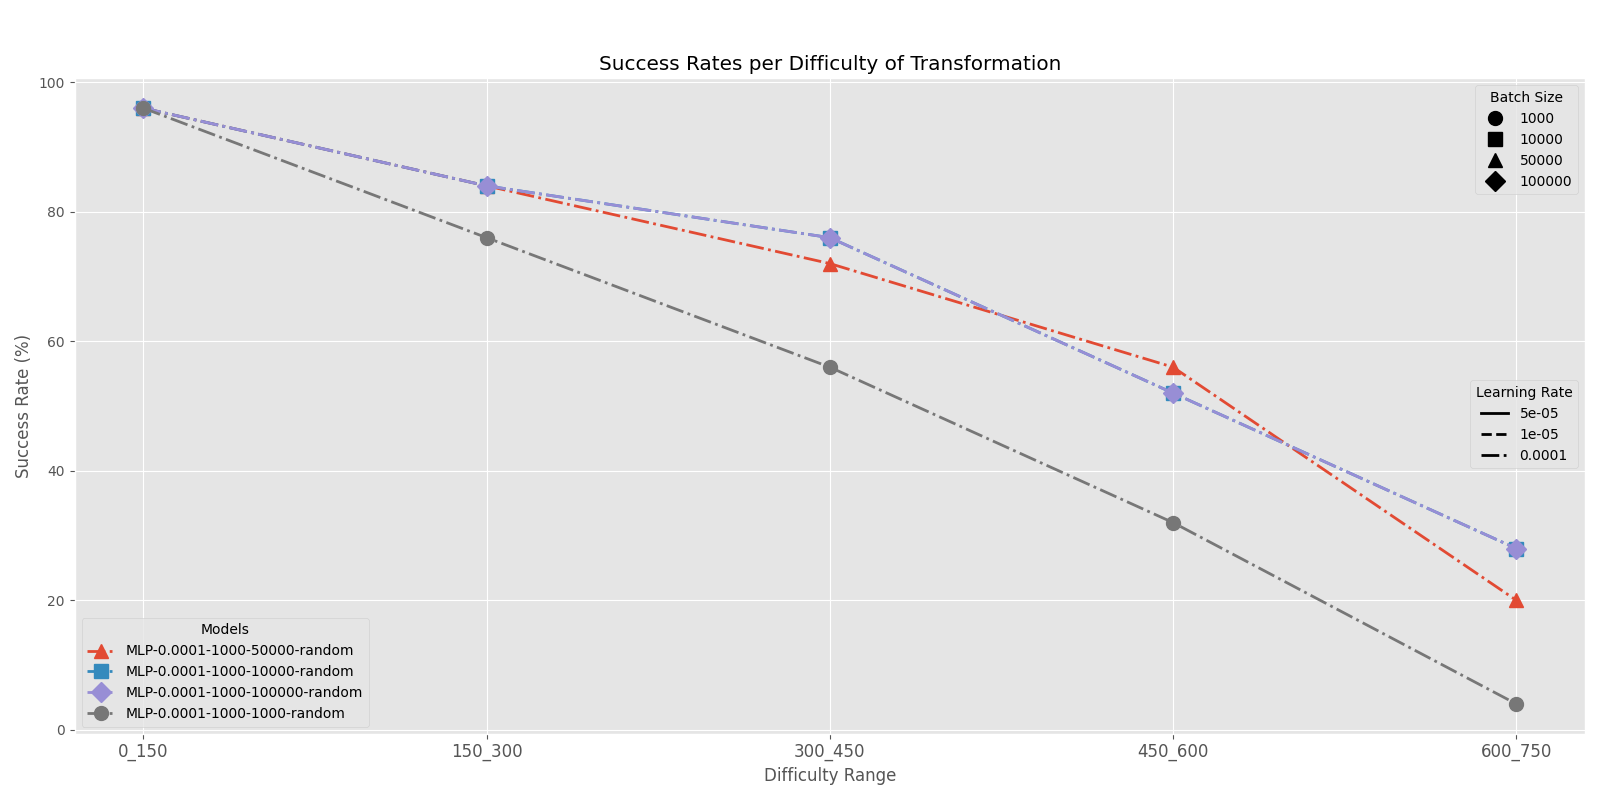
\includegraphics[width=0.8\textwidth]{imaxes/batchsize/experiment_plot_RFMID_MLP_0.0001.png}
    \caption{Comparación do rendemento da rede con diferentes batch sizes sobre imaxes do dataset RFMID ca función de activación ReLU (learning rate = 1e-4)}
    \label{fig:batch_size_comparison_relu_1e-4}
\end{figure}

\begin{figure}[ht] 
    \centering
    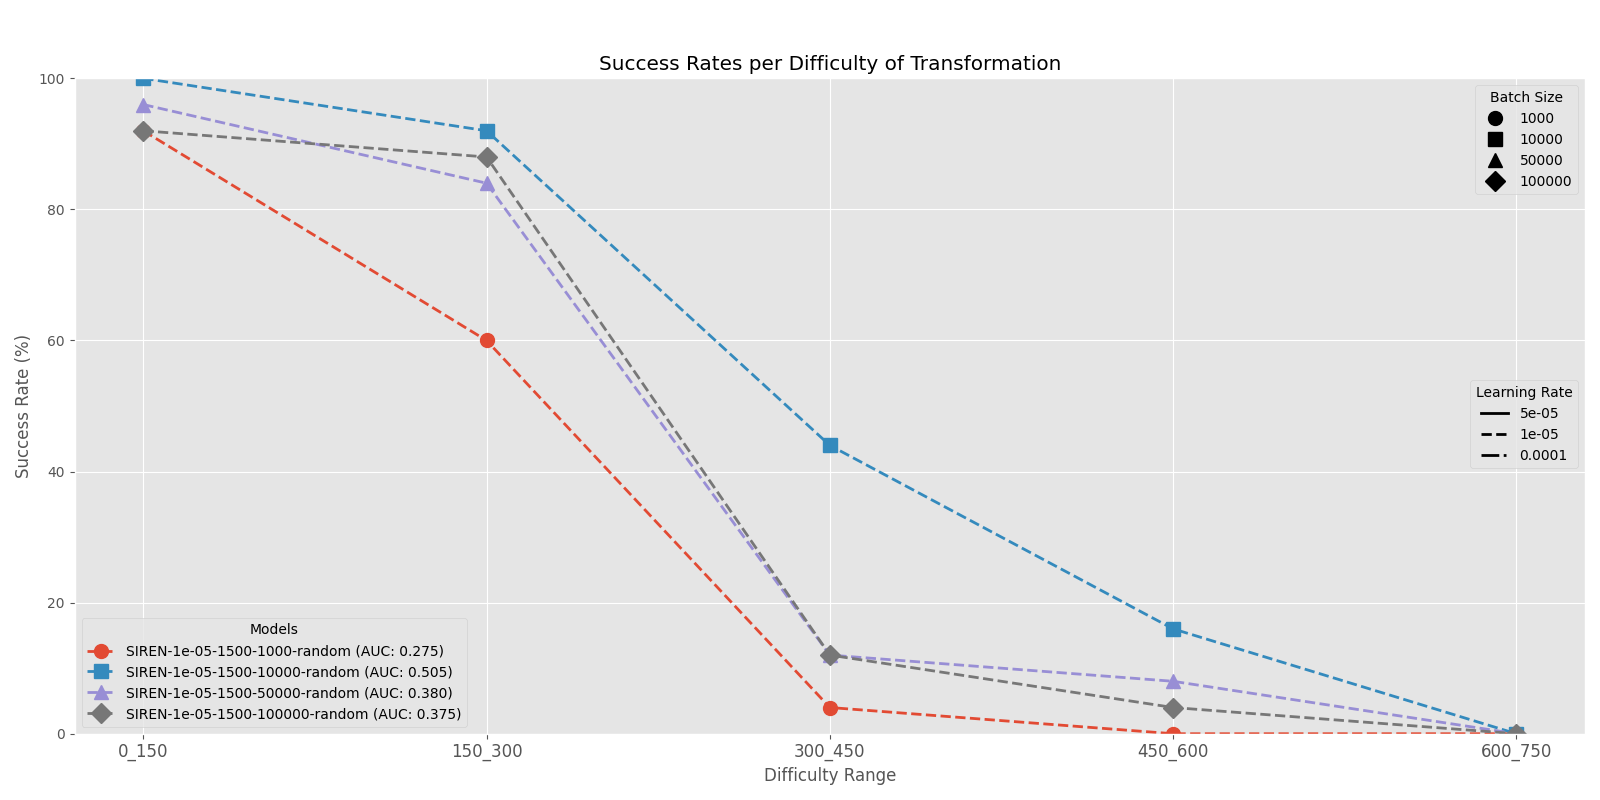
\includegraphics[width=0.8\textwidth]{imaxes/batchsize/experiment_plot_RFMID_SIREN_1e-05.png}
    \caption{Comparación do rendemento da rede con diferentes batch sizes sobre imaxes do dataset RFMID ca función de activación SIREN (learning rate = 1e-5)}
    \label{fig:batch_size_comparison_siren_1e-5}
\end{figure}

\begin{figure}[ht] 
    \centering
    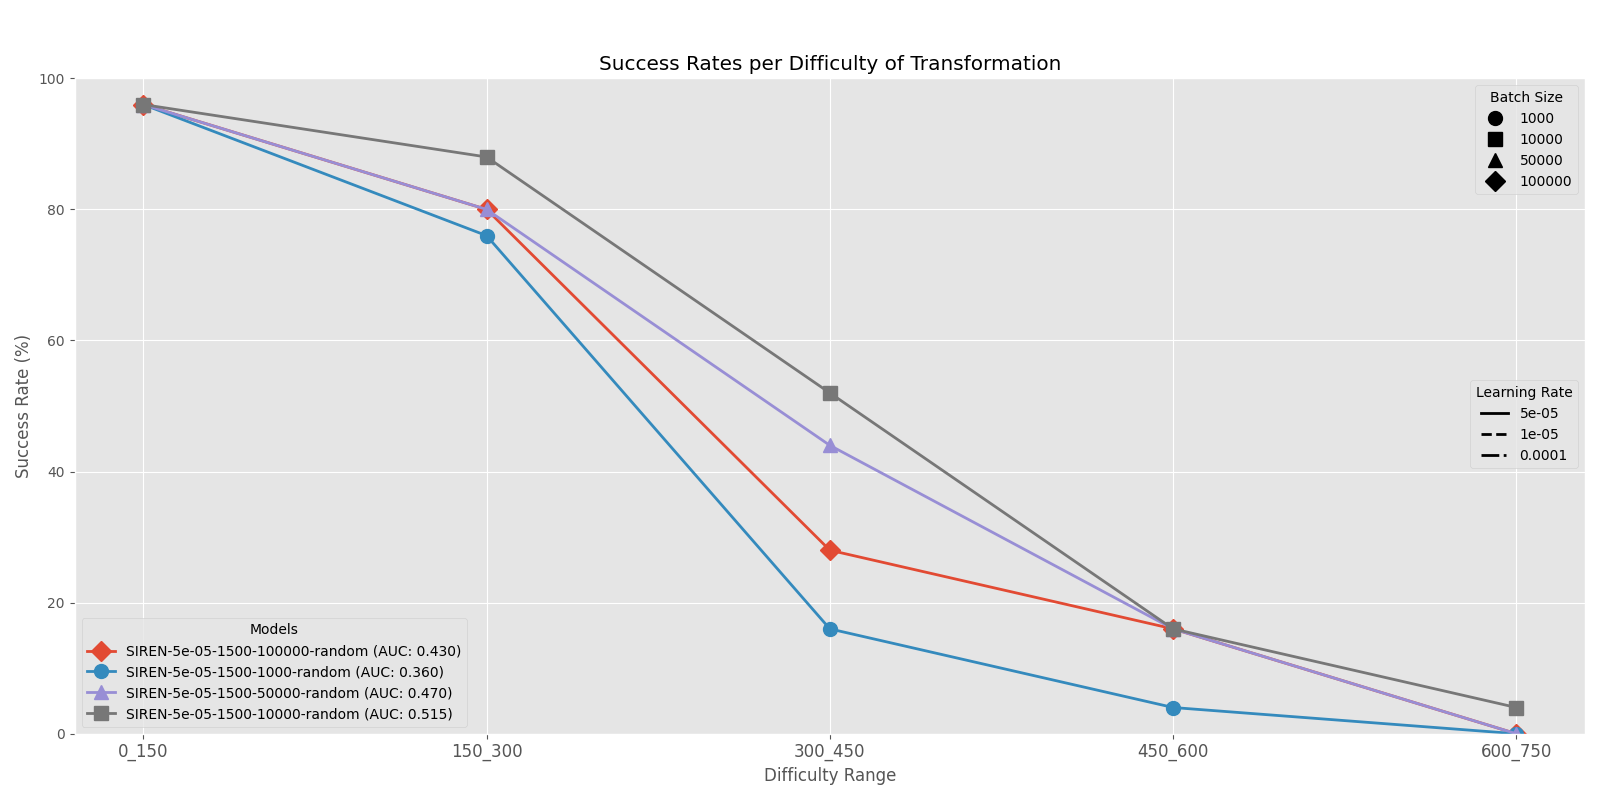
\includegraphics[width=0.8\textwidth]{imaxes/batchsize/experiment_plot_RFMID_SIREN_5e-05.png}
    \caption{Comparación do rendemento da rede con diferentes batch sizes sobre imaxes do dataset RFMID ca función de activación SIREN (learning rate = 5e-5)}
    \label{fig:batch_size_comparison_siren_5e-5}
\end{figure}

\begin{figure}[ht] 
    \centering
    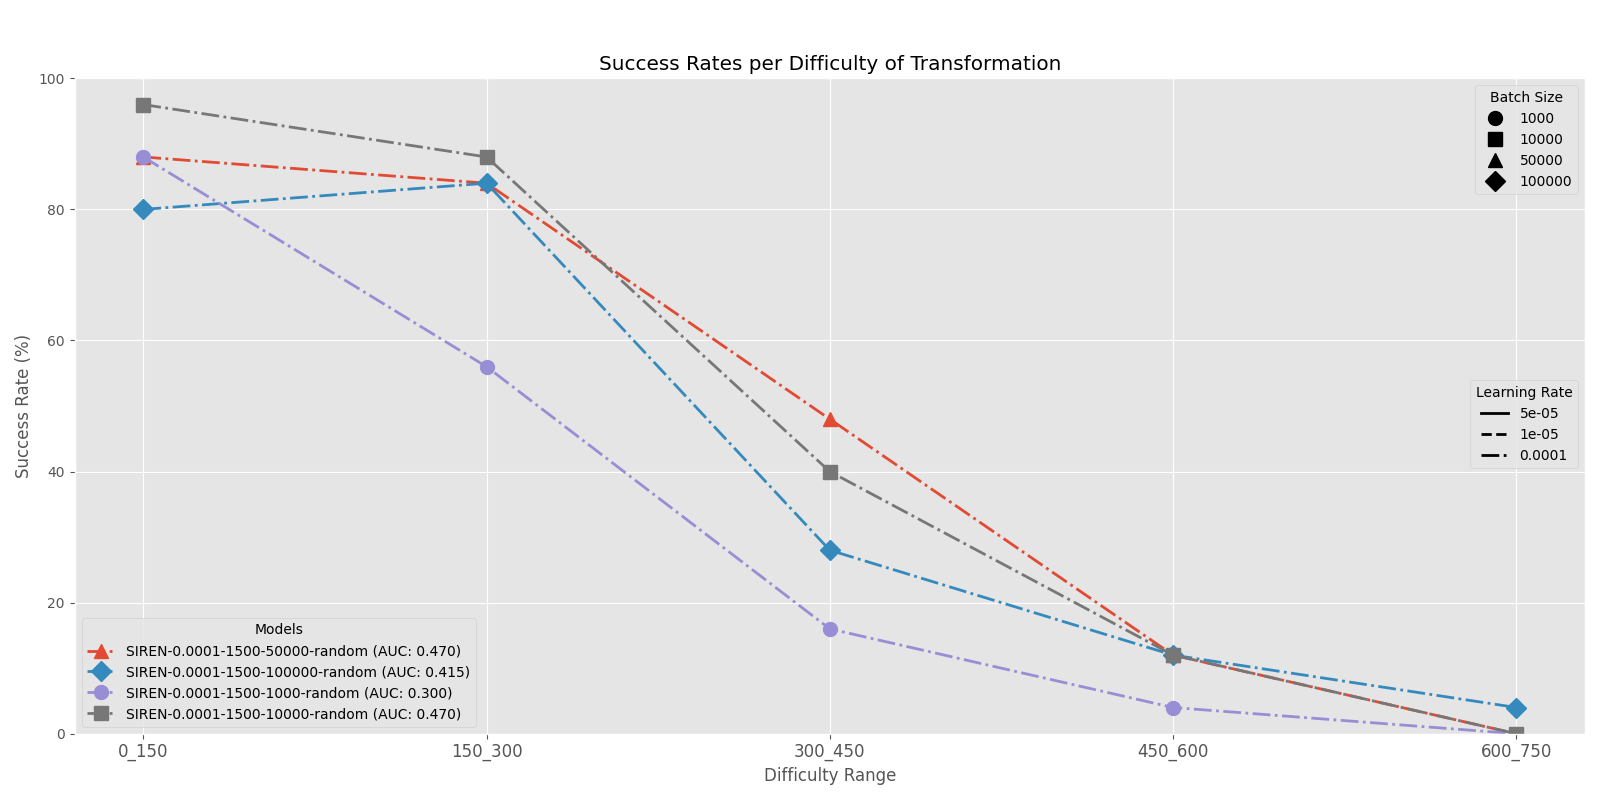
\includegraphics[width=0.8\textwidth]{imaxes/batchsize/experiment_plot_RFMID_SIREN_0.0001.png}
    \caption{Comparación do rendemento da rede con diferentes batch sizes sobre imaxes do dataset RFMID ca función de activación SIREN (learning rate = 1e-4)}
    \label{fig:batch_size_comparison_siren_1e-4}
\end{figure}


\paragraph{Discusión}
\label{par:Discusión}

Obsérvase que as redes ca función de activación ReLU tenden a ter un rendemento moito mellor que as ca función de activación SIREN. Isto pode explicarse xa que as deformacións artificiais que se aplican nas imaxes do dataset RFMID son lineais, e a función de activación ReLU é adecuada para este tipo de transformacións.

Tamén parece que o batch size é relevante, especialmente o cambio entre 1000 e 10000, mentres que batch sizes maiores (50000, 100000) non parecen ter tanto impacto, aínda que si un maior custo computacional.

\paragraph{Conclusións}
\label{par:Conclusións}

Interesa determinar cal é o punto de inflexión onde o aumento do batch size non compensa o aumento do rendemento.

\subsection{Estratexias de mostraxe}
\label{subsec:Estratexias de mostraxe}

Orixinalmente IDIR utiliza unha estratexia de mostraxe aleatoria para seleccionar os puntos que se pasan á rede en cada iteración.
Mentres que esta estratexia parece suficiente para o rexitro de pulmóns, no caso das imaxes de retina isto non ten porque ser así.
Isto débese a que as imaxes de retina conteñen seccións con moita mais información que outras, frente os CTs de pulmóns onde o sinal é mais uniforme.
Por exemplo, as seccións que conteñen vasos sanguíneos ou o disco óptico probablemente teñan mais información relevante para a tarefa de rexistro, frente outras seccións como o fondo da retina.
Ademais, as retinografías teñen desprazamentos moito maiores e menor superposición entre cada parella, polo que a rede ten que aprender transformacións mais complexas.

\paragraph{Planteamento}
\label{par:Planteamento}

Para solucionar isto, propúxose unha estratexia de mostraxe mais intellixente, onde se calcula unha máscara de probabilidade para cada imaxe, que se utiliza para seleccionar os puntos que se pasan á rede.
Para calcular esta máscara, extráense mediante operadores de Sobel os vasos sanguíneos e mediante umbralización o disco óptico, que son as zonas onde se espera que haxa máis información, e dáselles maiores probabilidades de ser seleccionadas.

Posteriormente tamén se introducíu unha estratexia de mostraxe uniforme, onde se seleccionan un número fixo de puntos en cada imaxe.
É unha estratexia similar ao mostraxe aleatorio, pero garantindo que se cubre a maior parte posible da imaxe. Isto é relevante en experimentos con batch sizes pequenos onde unha mostraxe aleatoria non ten por que cubrir toda a imaxe de forma uniforme.
Para implementalo empregouse unha distribución baseada na grella de Fibonacci (Fibonacci lattice), que permite repartir os puntos de maneira uniforme sobre a superficie circular da retina. 
A posición de cada punto calcúlase en coordenadas polares, asignando a cada punto un radio proporcional á raíz cadrada do seu índice dividido polo número total de puntos, e un ángulo proporcional ao índice multiplicado por $2\pi$ e dividido polo cadrado do número áureo ($\varphi^2$):

\[
r_i = \sqrt{\frac{i}{N}}, \quad \theta_i = 2\pi \frac{i}{\varphi^2}
\]

onde $i$ é o índice do punto ($i = 1, \dots, N$), $N$ é o número total de puntos e $\varphi$ é o número áureo. 
Deste xeito, conséguese unha cobertura uniforme e eficiente da rexión de interese, evitando agrupamentos ou zonas baleiras.

Así mesmo implementouse un scheduling do batch size, ca idea de utilizar un batch size pequeno nos epochs iniciais para que a rede aprenda unha transformación global a grandes rasgos, e aumentar o número de puntos conforme avanza o entrenamento para que a rede aprenda as transformación locais.
A estratexia de mostraxe uniforme é a mais axeitada para este caso, especialmente cando se utiliza un batch size pequeno.
O learning rate modificaráse de forma proporcional para manter a relación entre ambos.

Na figura \ref{fig:sampling_heatmaps} pódense observar os diferentes tipos de mostraxe utilizados.

\begin{figure}[]
    \centering
    \begin{subfigure}[b]{0.3\textwidth}
        \centering
        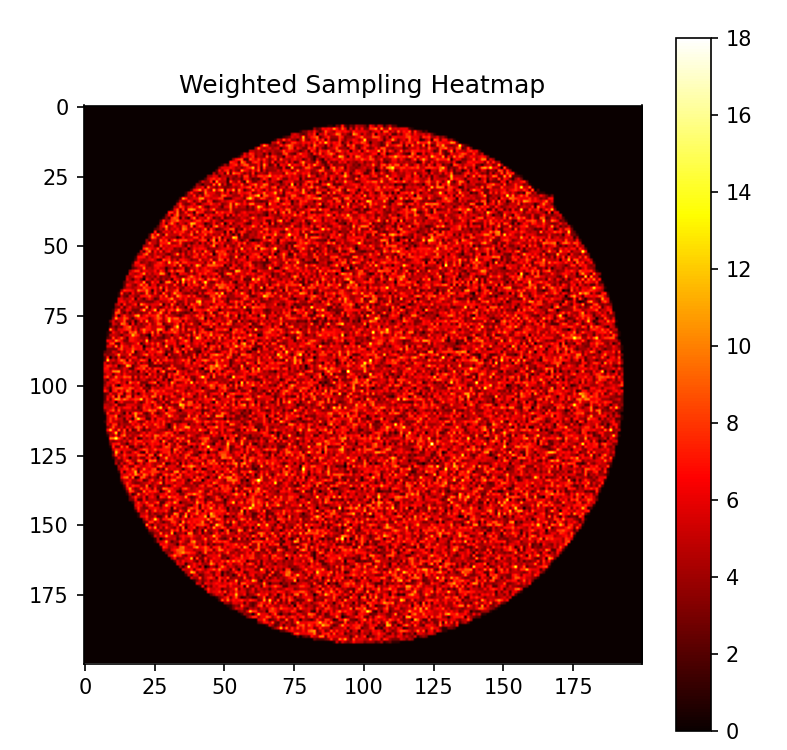
\includegraphics[width=\textwidth]{imaxes/muestraje/random_sampling_heatmap.png}
        \caption{Heatmap de mostraxe aleatorio}
        \label{fig:random_sampling_heatmap}
    \end{subfigure}
    \hfill
    \begin{subfigure}[b]{0.3\textwidth}
        \centering
        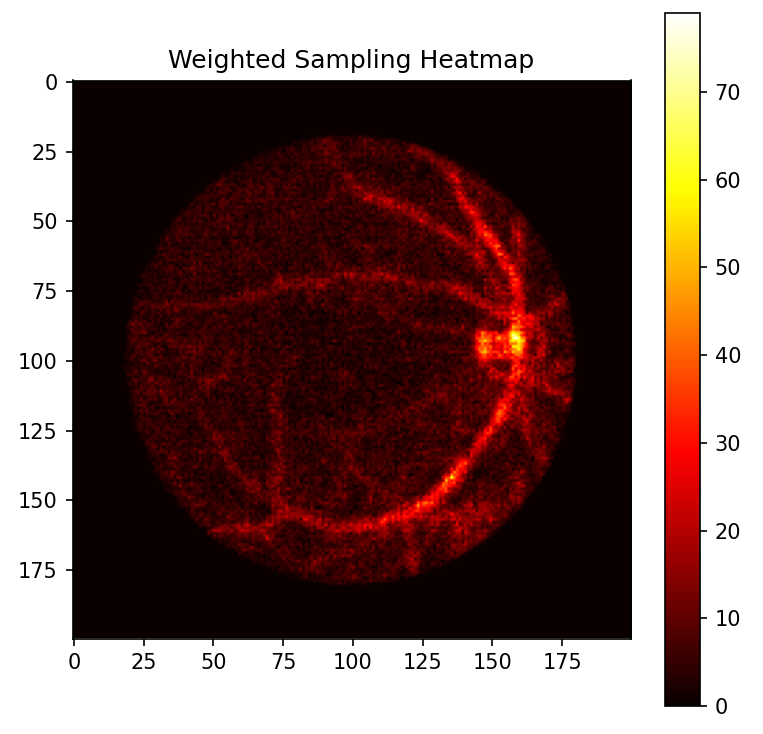
\includegraphics[width=\textwidth]{imaxes/muestraje/weighted_sampling_heatmap.png}
        \caption{Heatmap de mostraxe con peso}
        \label{fig:weighted_sampling_heatmap}
    \end{subfigure}
    \hfill
    \begin{subfigure}[b]{0.3\textwidth}
        \centering
        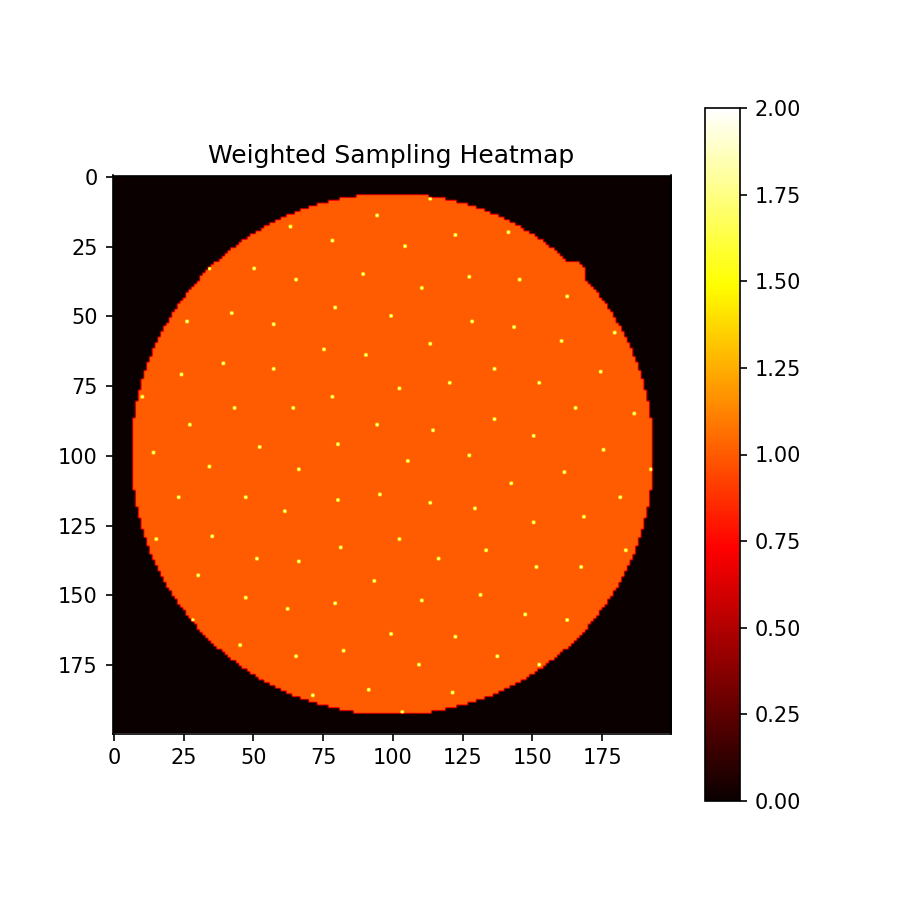
\includegraphics[width=\textwidth]{imaxes/muestraje/uniform_sampling_heatmap.png}
        \caption{Heatmap de mostraxe uniforme (100 puntos)}
        \label{fig:uniform_sampling_heatmap}
    \end{subfigure}
    \caption{Heatmaps de mostraxe}
    \label{fig:sampling_heatmaps}
\end{figure}


\paragraph{Resultados}
\label{par:Resultados}

\ref{fig:sampling_comparison}
\ref{fig:fire_samplingtype}
\ref{fig:sampling_comparison_relu}
\ref{fig:sampling_comparison_SIREN}
\begin{figure}[ht]
    \centering
    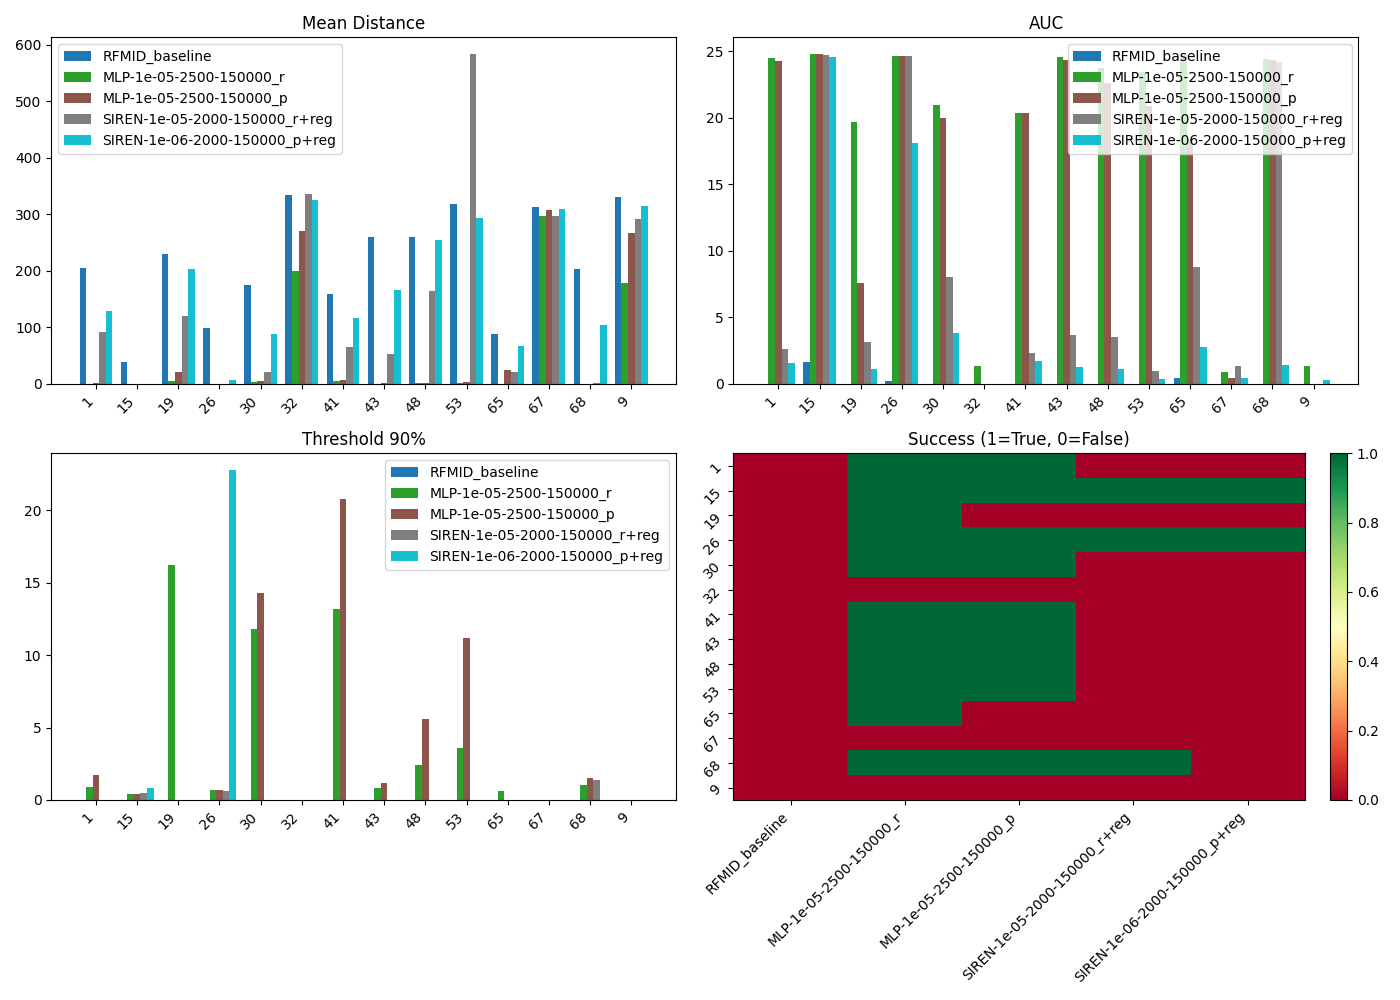
\includegraphics[width=0.8\textwidth]{imaxes/muestraje/RFMID_both__comp_sampling.png}
    \caption{Comparación das diferentes estratexias de mostraxe sobre imaxes do dataset RFMID}
    \label{fig:sampling_comparison}
\end{figure}

\begin{figure}[ht]
    \centering
    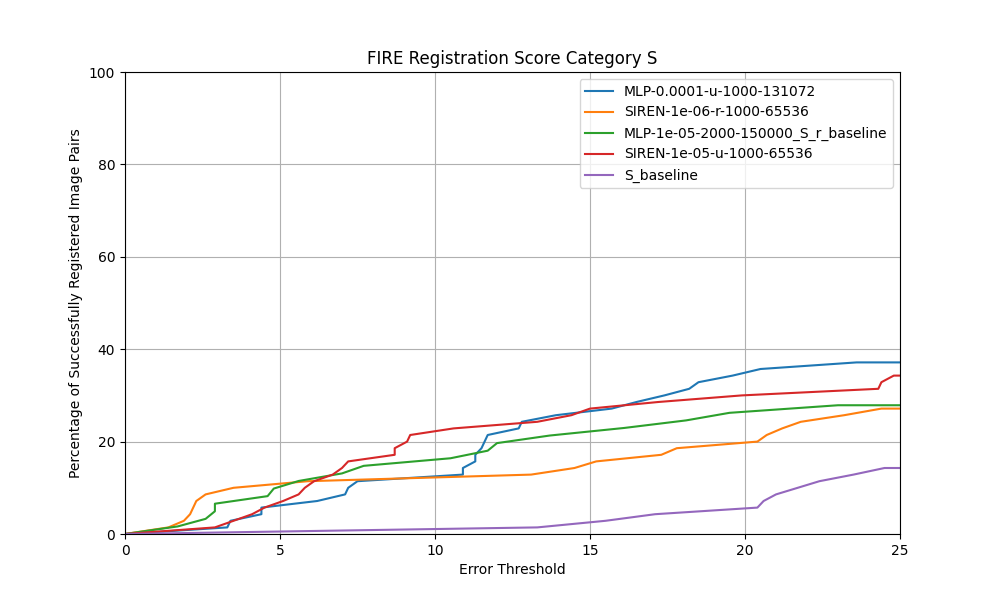
\includegraphics[width=0.8\textwidth]{imaxes/muestraje/fire_samplingtype.png}
    \caption{Comparación das diferentes estratexias de mostraxe sobre imaxes do dataset FIRE}
    \label{fig:fire_samplingtype}
\end{figure}


\begin{figure}[ht]
    \centering
    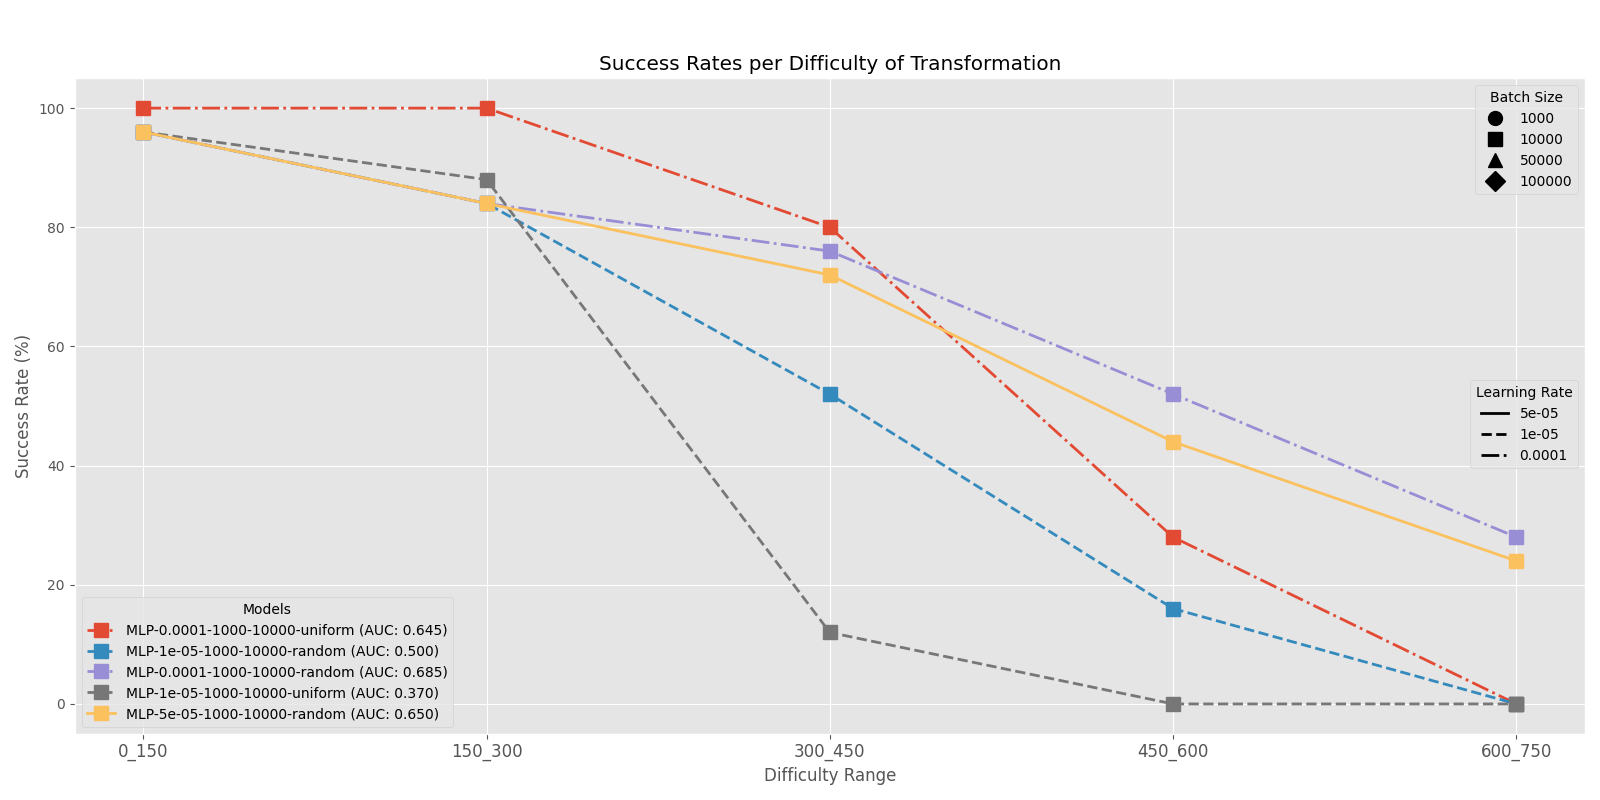
\includegraphics[width=0.8\textwidth]{imaxes/muestraje/experiment_plot_RFMID_MLP_RvsU.png}
    \caption{Comparación das diferentes estratexias de mostraxe sobre imaxes do dataset RFMID ca función de activación RELU}
    \label{fig:sampling_comparison_relu}
\end{figure}

\begin{figure}[ht]
    \centering
    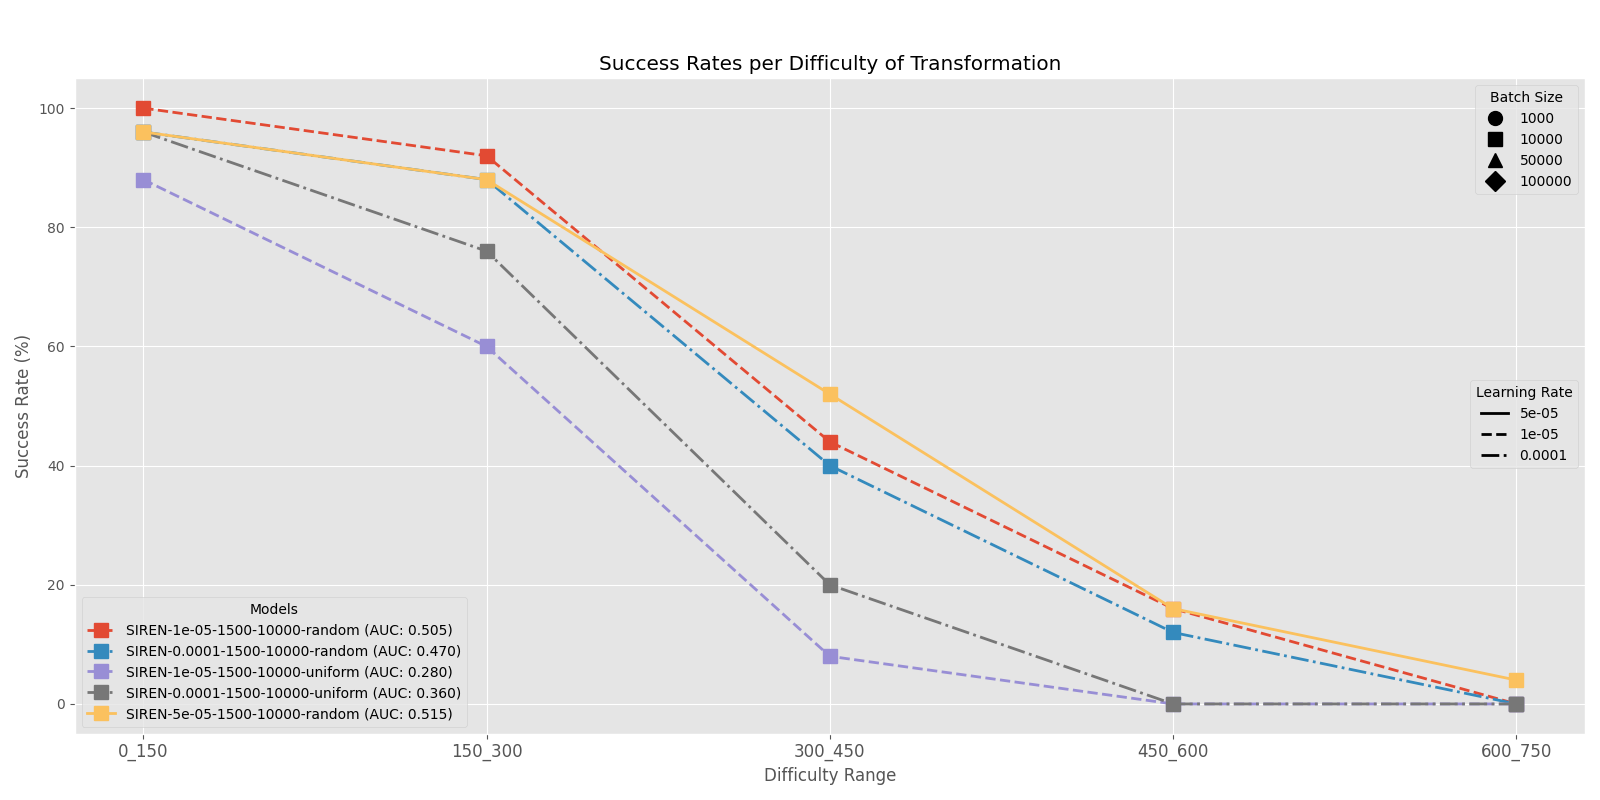
\includegraphics[width=0.8\textwidth]{imaxes/muestraje/experiment_plot_RFMID_SIREN_RvsU.png}
    \caption{Comparación das diferentes estratexias de mostraxe sobre imaxes do dataset RFMID ca función de activación SIREN}
    \label{fig:sampling_comparison_SIREN}
\end{figure}



\paragraph{Discusión}
\label{par:Discusión}

A hipótese da estratexia de mostraxe intellixente non parece ser a mais axeitada, con resultados peores ca estratexia aleatoria. 
A estratexia uniforme tampouco parece ser a mais adecuada, xa que non se obtén resultados significativamente mellores ca a aleatoria.


\paragraph{Conclusións}
\label{par:Conclusións}

\subsection{Inicialización}
\label{subsec:Inicialización}



\paragraph{Planteamento}
\label{par:Planteamento}

É posible que a inicialización da rede sexa un factor mais importante que a estratexia de mostraxe. É posible que certas inicializacións coloquen os despraszamentos de forma que a rede sexa incapaz de aprender a transformación correcta, ou que lle custe moito mais aprenderla.

Para testar esta hipótese implementouse unha lotería de inicialización, onde se utiliza o loss no epoch 0 para determinar a inicialización da rede mais beneficiosa.
É posible que fore mellor esperar ata un epoch algo mais avanzado para determinar a inicialización, xa que no epoch 0 non hay ningunha seguridade de que non sexa un mínimo local, pero isto tamén implicaría un maior custo computacional.

\paragraph{Resultados}
\label{par:Resultados}

\ref{fig:lottery_initial_deformations_combinedMLP}, \ref{fig:lottery_initial_deformations_combinedSIREN}

\begin{figure}[ht]
    \centering
    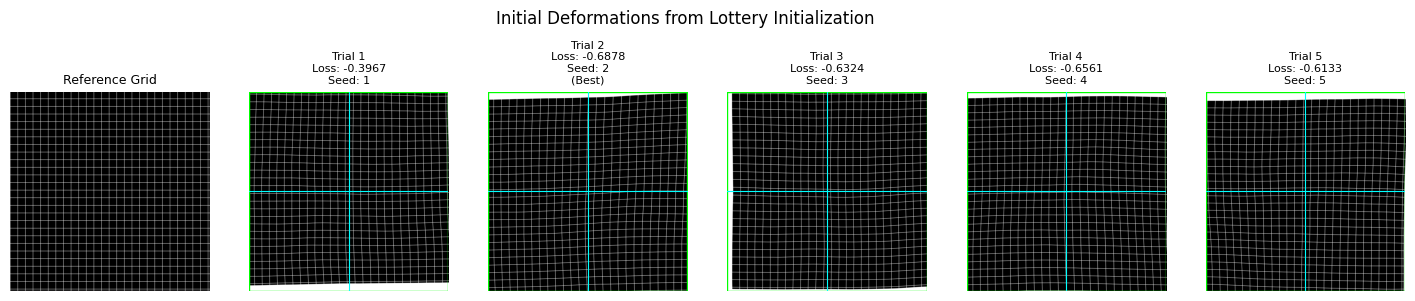
\includegraphics[width=0.8\textwidth]{imaxes/lottery/initial_deformations_combinedMLP.png}
    \caption{Exemplos das diferentes inicializacións ca función de activación RELU}
    \label{fig:lottery_initial_deformations_combinedMLP}
\end{figure}

\begin{figure}[ht]
    \centering
    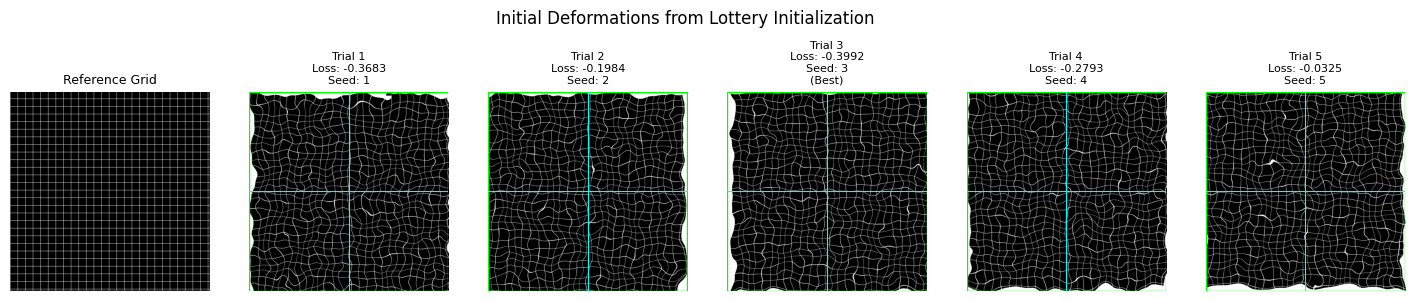
\includegraphics[width=0.8\textwidth]{imaxes/lottery/initial_deformations_combinedSIREN.png}
    \caption{Exemplos das diferentes inicializacións ca función de activación SIREN}
    \label{fig:lottery_initial_deformations_combinedSIREN}
\end{figure}

\paragraph{Discusión}
\label{par:Discusión}

\paragraph{Conclusións}
\label{par:Conclusións}

\subsection{Exemplos de rexistro}
\label{subsec:Exemplos de rexistro}

\ref{fig:reg_examples}

Estes exemplos ilustran o resultado do rexistro de diferentes imaxes, mostrando tanto rexistros exitosos como fallidos.
A primeira imaxe corresponde ca imaxe fixa, a segunda corresponde ca imaxe rexistrada, a terceira ca imaxe móbil e a cuarta o campos de deformación aplicado a unha gralla cadrada.

Pódense observar os puntos de control, sendo os blancos os da imaxe fixa, os verdes os da imaxe móbil e os azuis os desprazados pola rede.
\begin{figure}[ht]
    \centering
    \begin{subfigure}[b]{0.45\textwidth}
        \centering
        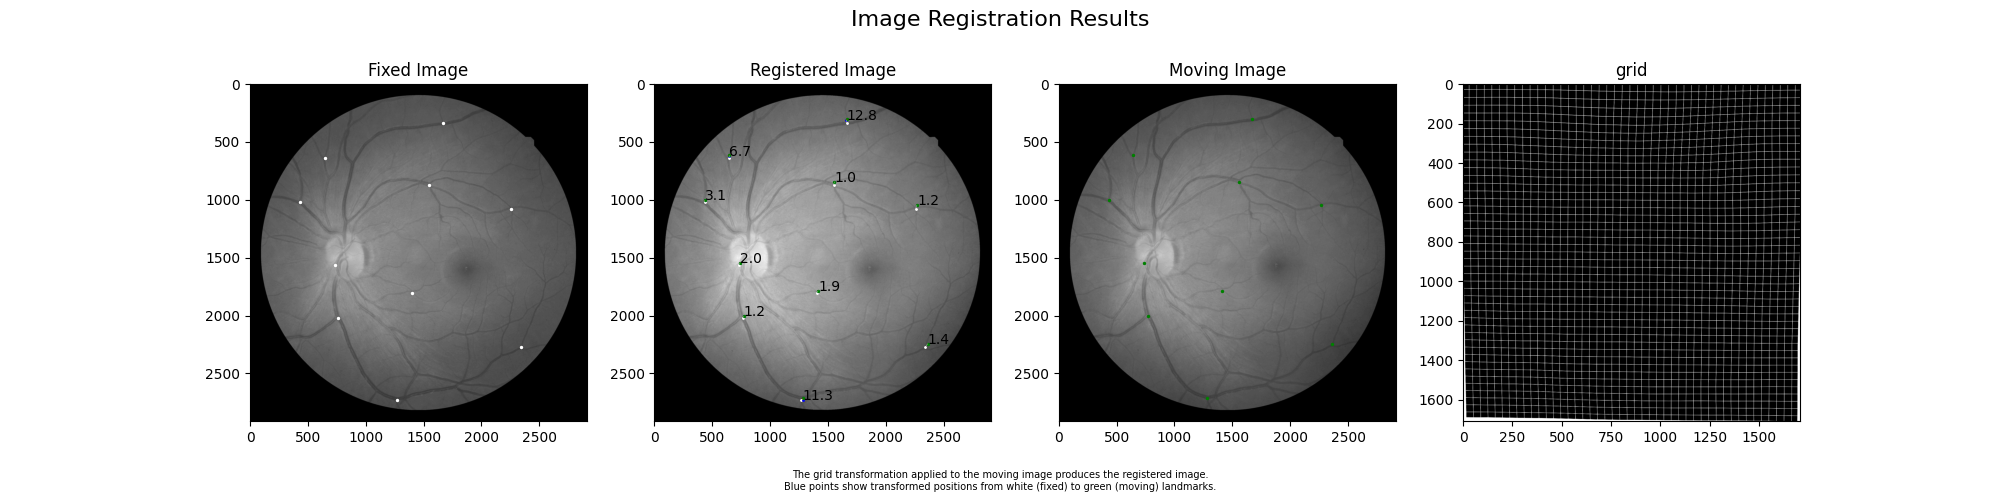
\includegraphics[width=\textwidth]{imaxes/reg_examples/FIRE_MLP_buena.png}
        \caption{Rexistro exitoso dunha parella de imaxes do dataset FIRE ca función de activación ReLU}
        \label{fig:reg_example_FIRE_MLP_buena}
    \end{subfigure}\hfill
    \begin{subfigure}[b]{0.45\textwidth}
        \centering
        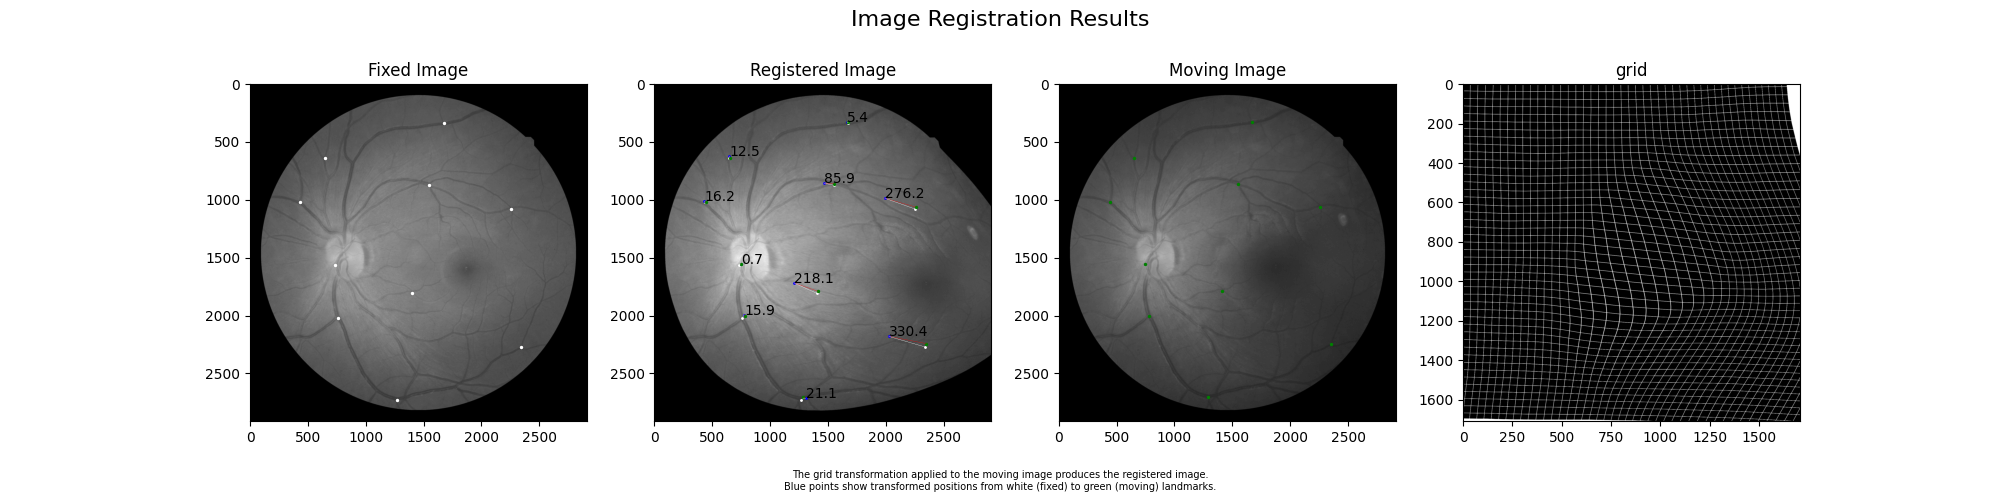
\includegraphics[width=\textwidth]{imaxes/reg_examples/FIRE_MLP_mala.png}
        \caption{Rexistro fallido dunha parella de imaxes do dataset FIRE ca función de activación ReLU}
        \label{fig:reg_example_FIRE_MLP_mala}
    \end{subfigure}

    \vskip\baselineskip

    \begin{subfigure}[b]{0.45\textwidth}
        \centering
        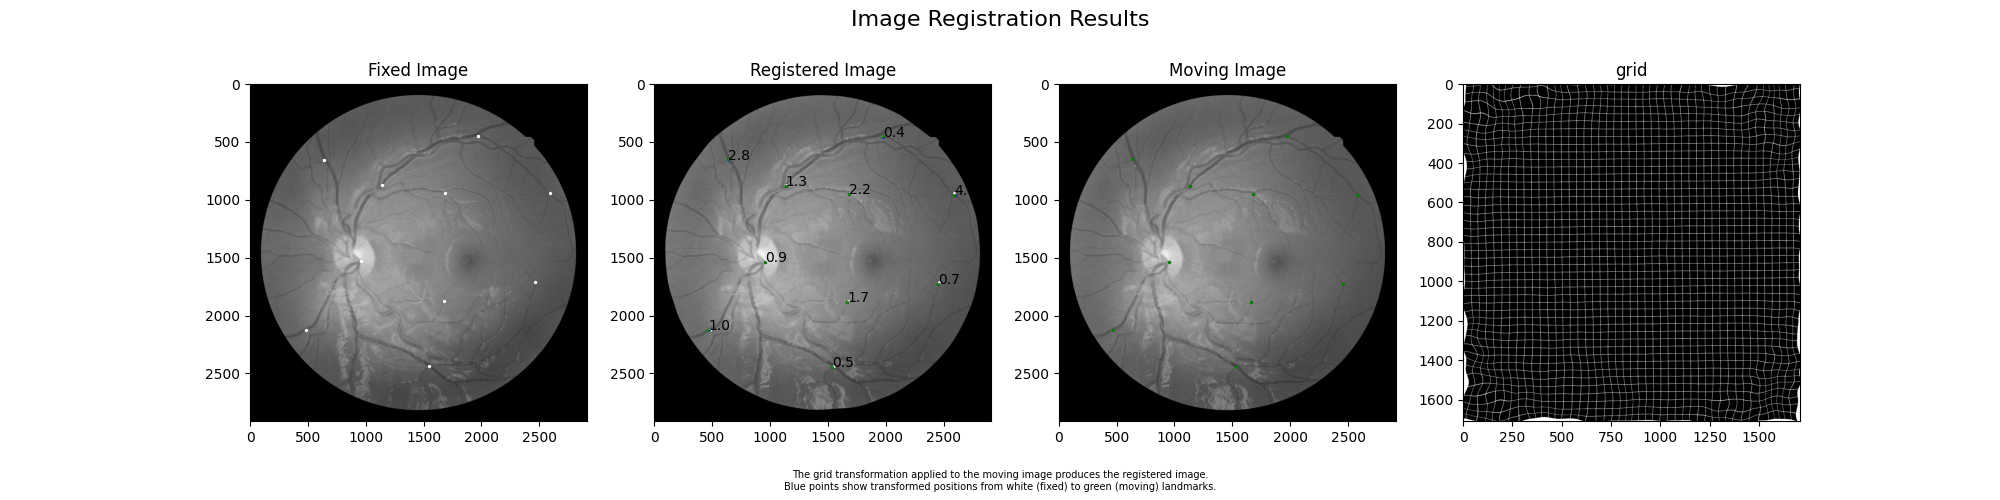
\includegraphics[width=\textwidth]{imaxes/reg_examples/FIRE_SIREN_buena.png}
        \caption{Rexistro exitoso dunha parella de imaxes do dataset FIRE ca función de activación SIREN}
        \label{fig:reg_example_FIRE_SIREN_buena}
    \end{subfigure}\hfill
    \begin{subfigure}[b]{0.45\textwidth}
        \centering
        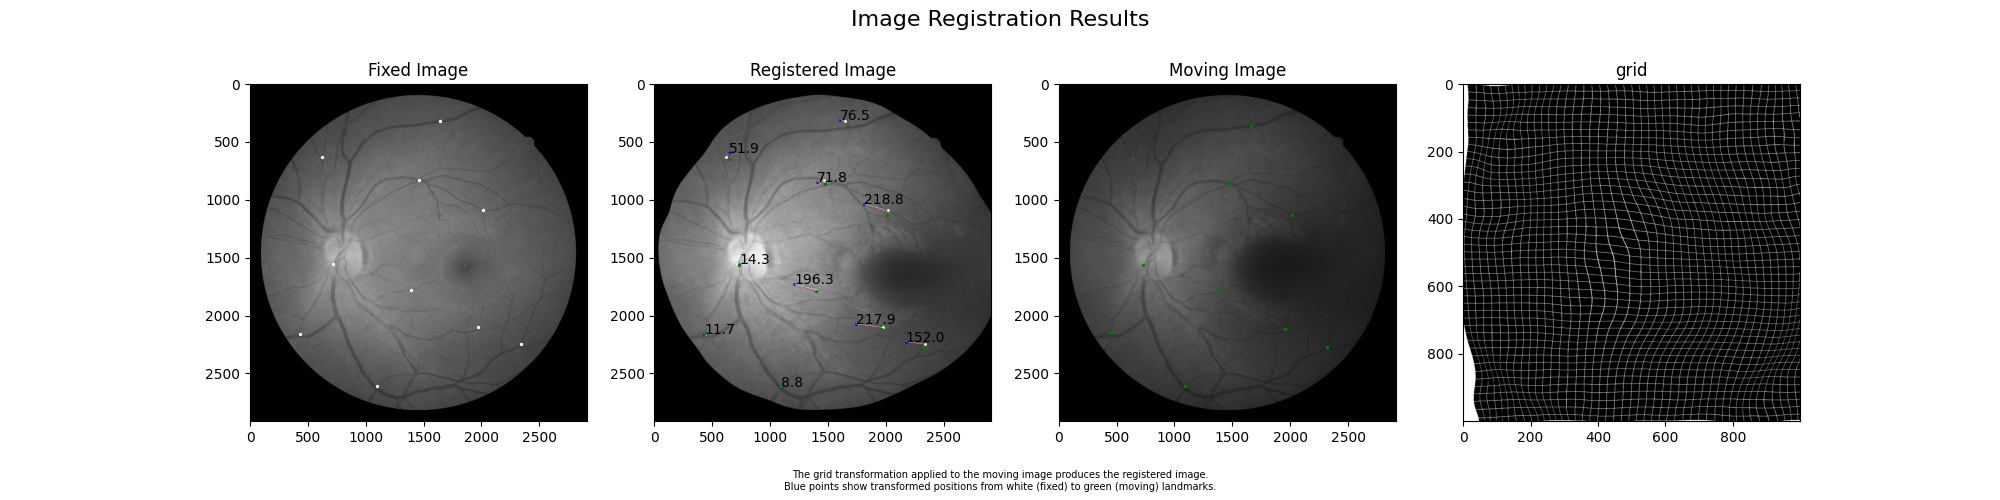
\includegraphics[width=\textwidth]{imaxes/reg_examples/FIRE_SIREN_mala.png}
        \caption{Rexistro fallido dunha parella de imaxes do dataset FIRE ca función de activación SIREN}
        \label{fig:reg_example_FIRE_SIREN_mala}
    \end{subfigure}

    \vskip\baselineskip

    \begin{subfigure}[b]{0.45\textwidth}
        \centering
        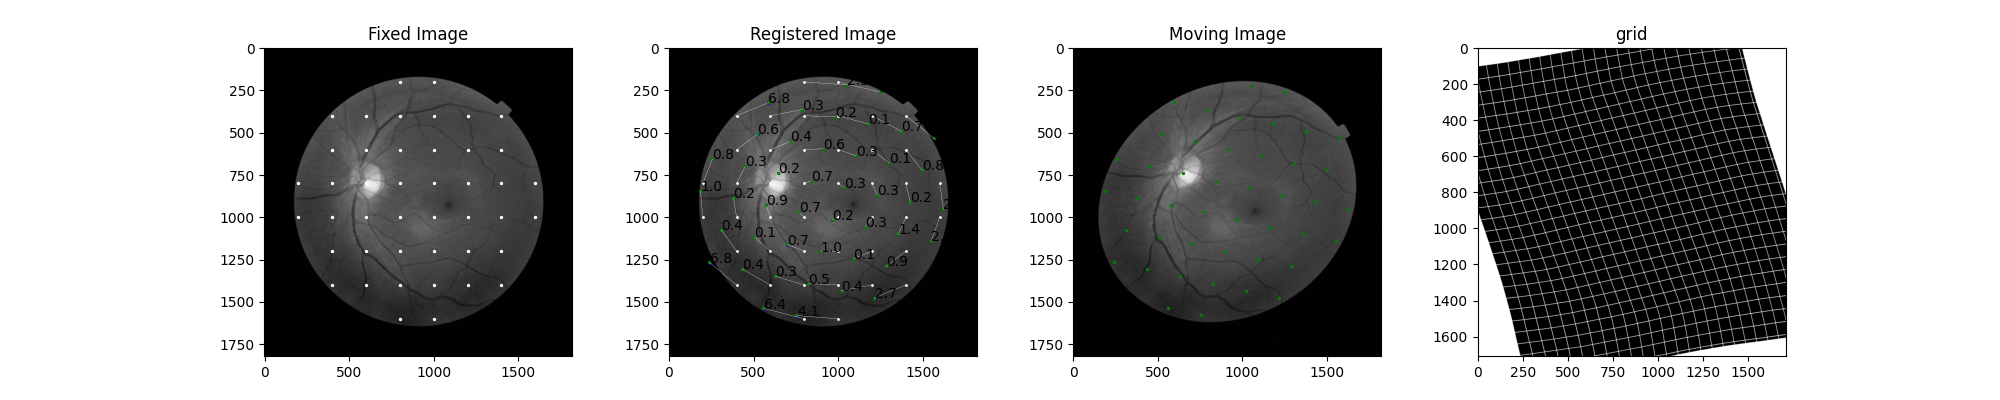
\includegraphics[width=\textwidth]{imaxes/reg_examples/RFMID_MLP_buena.png}
        \caption{Rexistro exitoso dunha parella de imaxes do dataset RFMID ca función de activación ReLU}
        \label{fig:reg_example_RFMID_MLP_buena}
    \end{subfigure}\hfill
    \begin{subfigure}[b]{0.45\textwidth}
        \centering
        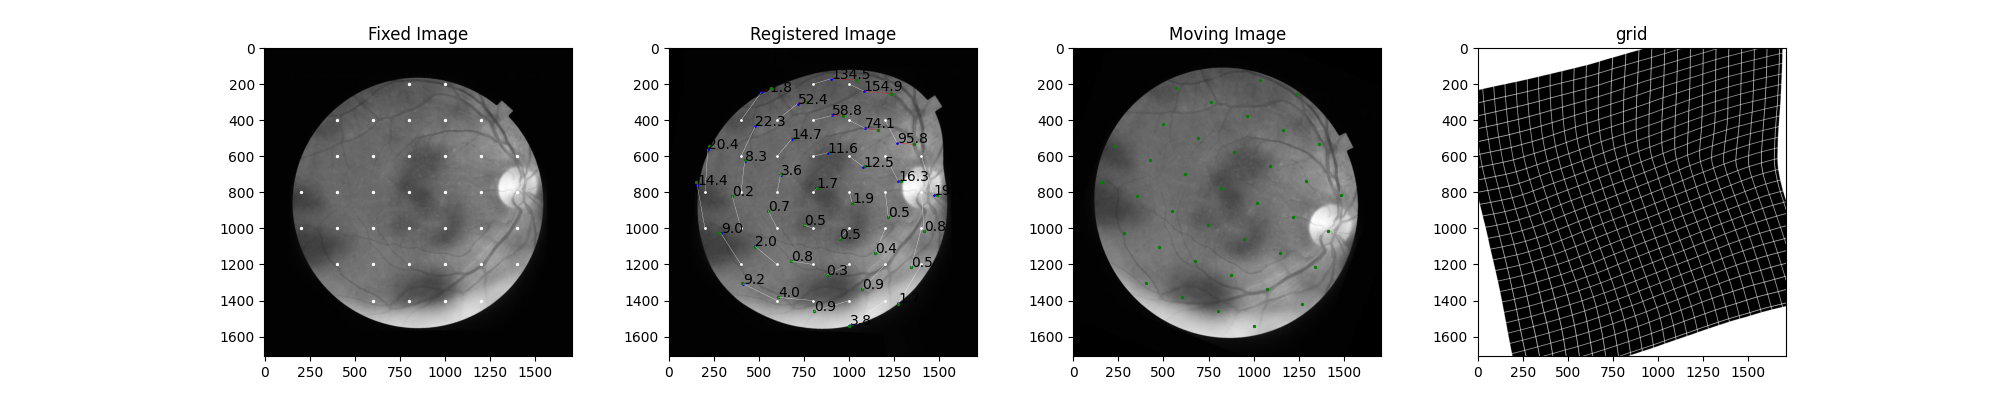
\includegraphics[width=\textwidth]{imaxes/reg_examples/RFMID_MLP_mala.png}
        \caption{Rexistro fallido dunha parella de imaxes do dataset RFMID ca función de activación ReLU}
        \label{fig:reg_example_RFMID_MLP_mala}
    \end{subfigure}

    \vskip\baselineskip

    \begin{subfigure}[b]{0.45\textwidth}
        \centering
        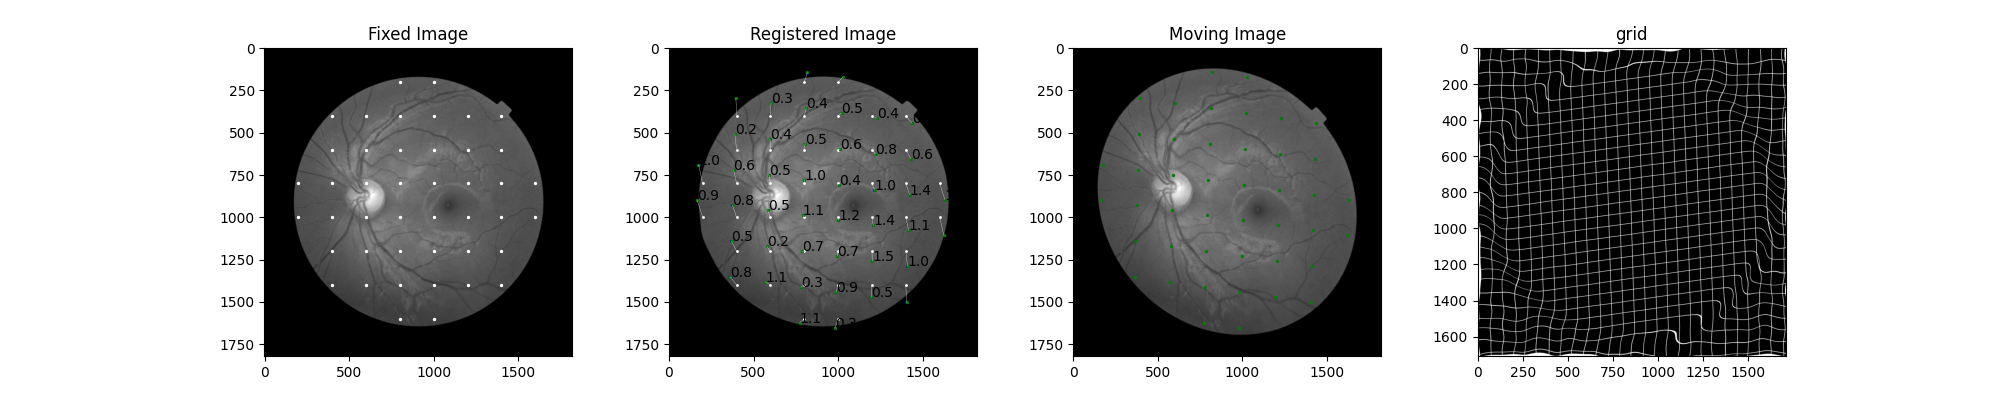
\includegraphics[width=\textwidth]{imaxes/reg_examples/RFMID_SIREN_buena.png}
        \caption{Rexistro exitoso dunha parella de imaxes do dataset RFMID ca función de activación SIREN}
        \label{fig:reg_example_RFMID_SIREN_buena}
    \end{subfigure}\hfill
    \begin{subfigure}[b]{0.45\textwidth}
        \centering
        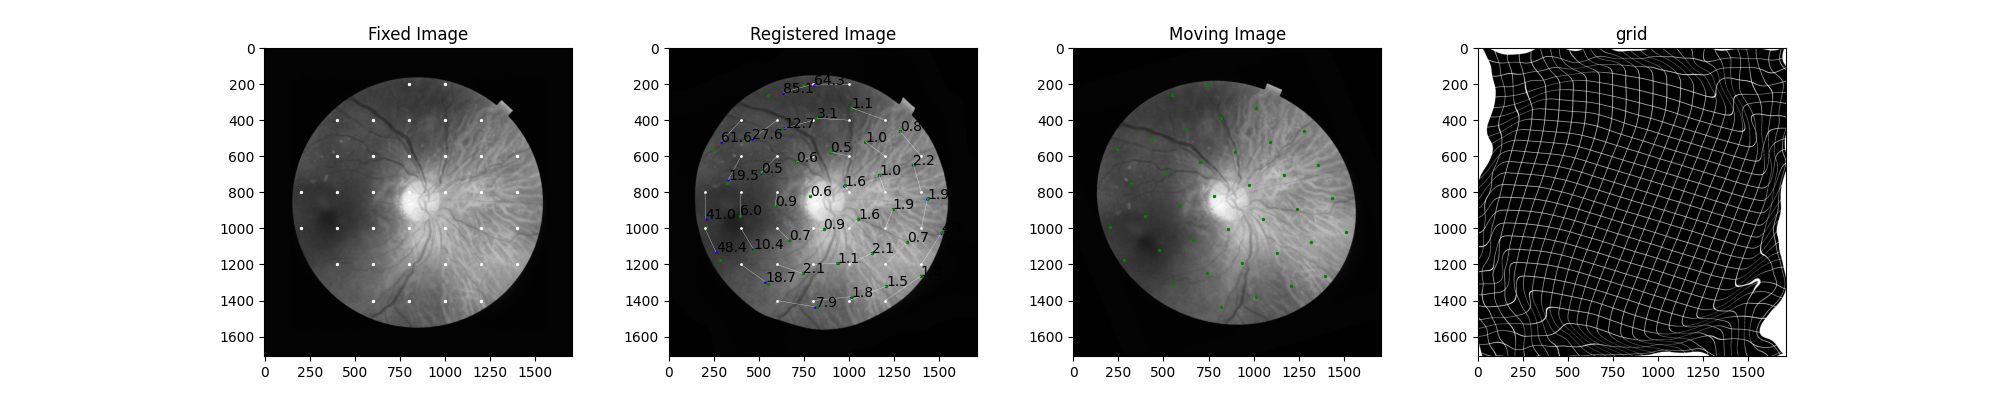
\includegraphics[width=\textwidth]{imaxes/reg_examples/RFMID_SIREN_mala.png}
        \caption{Rexistro fallido dunha parella de imaxes do dataset RFMID ca función de activación SIREN}
        \label{fig:reg_example_RFMID_SIREN_mala}
    \end{subfigure}

    \caption{Exemplos de rexistro: combinacións de dataset (FIRE/RFMID), función de activatción (relu/SIREN) e éxito.}
    \label{fig:reg_examples}
\end{figure}